\documentclass[12pt, oneside, openany]{book}

% ── Encoding & Font ──────────────────────────────────────────────────────────
\usepackage{fontspec}
\setmainfont{TeX Gyre Pagella}
\setsansfont{TeX Gyre Heros}
\setmonofont{TeX Gyre Cursor}

% ── Page geometry ────────────────────────────────────────────────────────────
\usepackage[
  paperwidth=6in,
  paperheight=9in,
  top=0.85in,
  bottom=0.85in,
  inner=0.75in,
  outer=0.65in
]{geometry}

% ── Tables ───────────────────────────────────────────────────────────────────
\usepackage{longtable}
\usepackage{booktabs}
\usepackage{array}
\usepackage{ragged2e}
\usepackage{xltabular}
\setlength{\LTpre}{6pt}
\setlength{\LTpost}{6pt}

% ── Colour, graphics ─────────────────────────────────────────────────────────
\usepackage{graphicx}
\usepackage{xcolor}

% ── Typography ───────────────────────────────────────────────────────────────
\usepackage{microtype}
\usepackage{setspace}
\setstretch{1.15}
\setlength{\parindent}{1.5em}
\setlength{\parskip}{0pt}

% ── Headers and footers ──────────────────────────────────────────────────────
\usepackage{fancyhdr}
\pagestyle{fancy}
\fancyhf{}
\fancyhead[L]{\small\itshape\leftmark}
\fancyhead[R]{\small\thepage}
\renewcommand{\headrulewidth}{0.3pt}
\fancypagestyle{plain}{
  \fancyhf{}
  \fancyfoot[C]{\small\thepage}
  \renewcommand{\headrulewidth}{0pt}
}

% ── Chapter titles ───────────────────────────────────────────────────────────
\usepackage{titlesec}
\titleformat{\chapter}[display]
  {\normalfont\large\bfseries\centering}
  {\chaptertitlename\ \thechapter}
  {12pt}
  {\LARGE}
\titlespacing*{\chapter}{0pt}{30pt}{20pt}

% ── Hyperlinks ───────────────────────────────────────────────────────────────
\usepackage[
  colorlinks=true,
  linkcolor=black,
  urlcolor=black,
  citecolor=black,
  pdftitle={Cartomantic Practices for Practical Use},
  pdfauthor={},
  bookmarks=true
]{hyperref}

% ── Bibliography ─────────────────────────────────────────────────────────────
\usepackage[backend=biber, style=authoryear, sorting=nyt]{biblatex}
\addbibresource{references.bib}

% ── Pandoc compatibility ─────────────────────────────────────────────────────
\providecommand{\tightlist}{\setlength{\itemsep}{0pt}\setlength{\parskip}{0pt}}

% ── Misc ─────────────────────────────────────────────────────────────────────
\setlength{\headheight}{14pt}
\usepackage{emptypage}
\usepackage{tocloft}
\renewcommand{\cftchapfont}{\normalfont}
\renewcommand{\cftchappagefont}{\normalfont}

% ─────────────────────────────────────────────────────────────────────────────
\begin{document}

% ── Cover ────────────────────────────────────────────────────────────────────
\begin{titlepage}
  \thispagestyle{empty}
  \begin{center}
    \vspace*{\fill}
    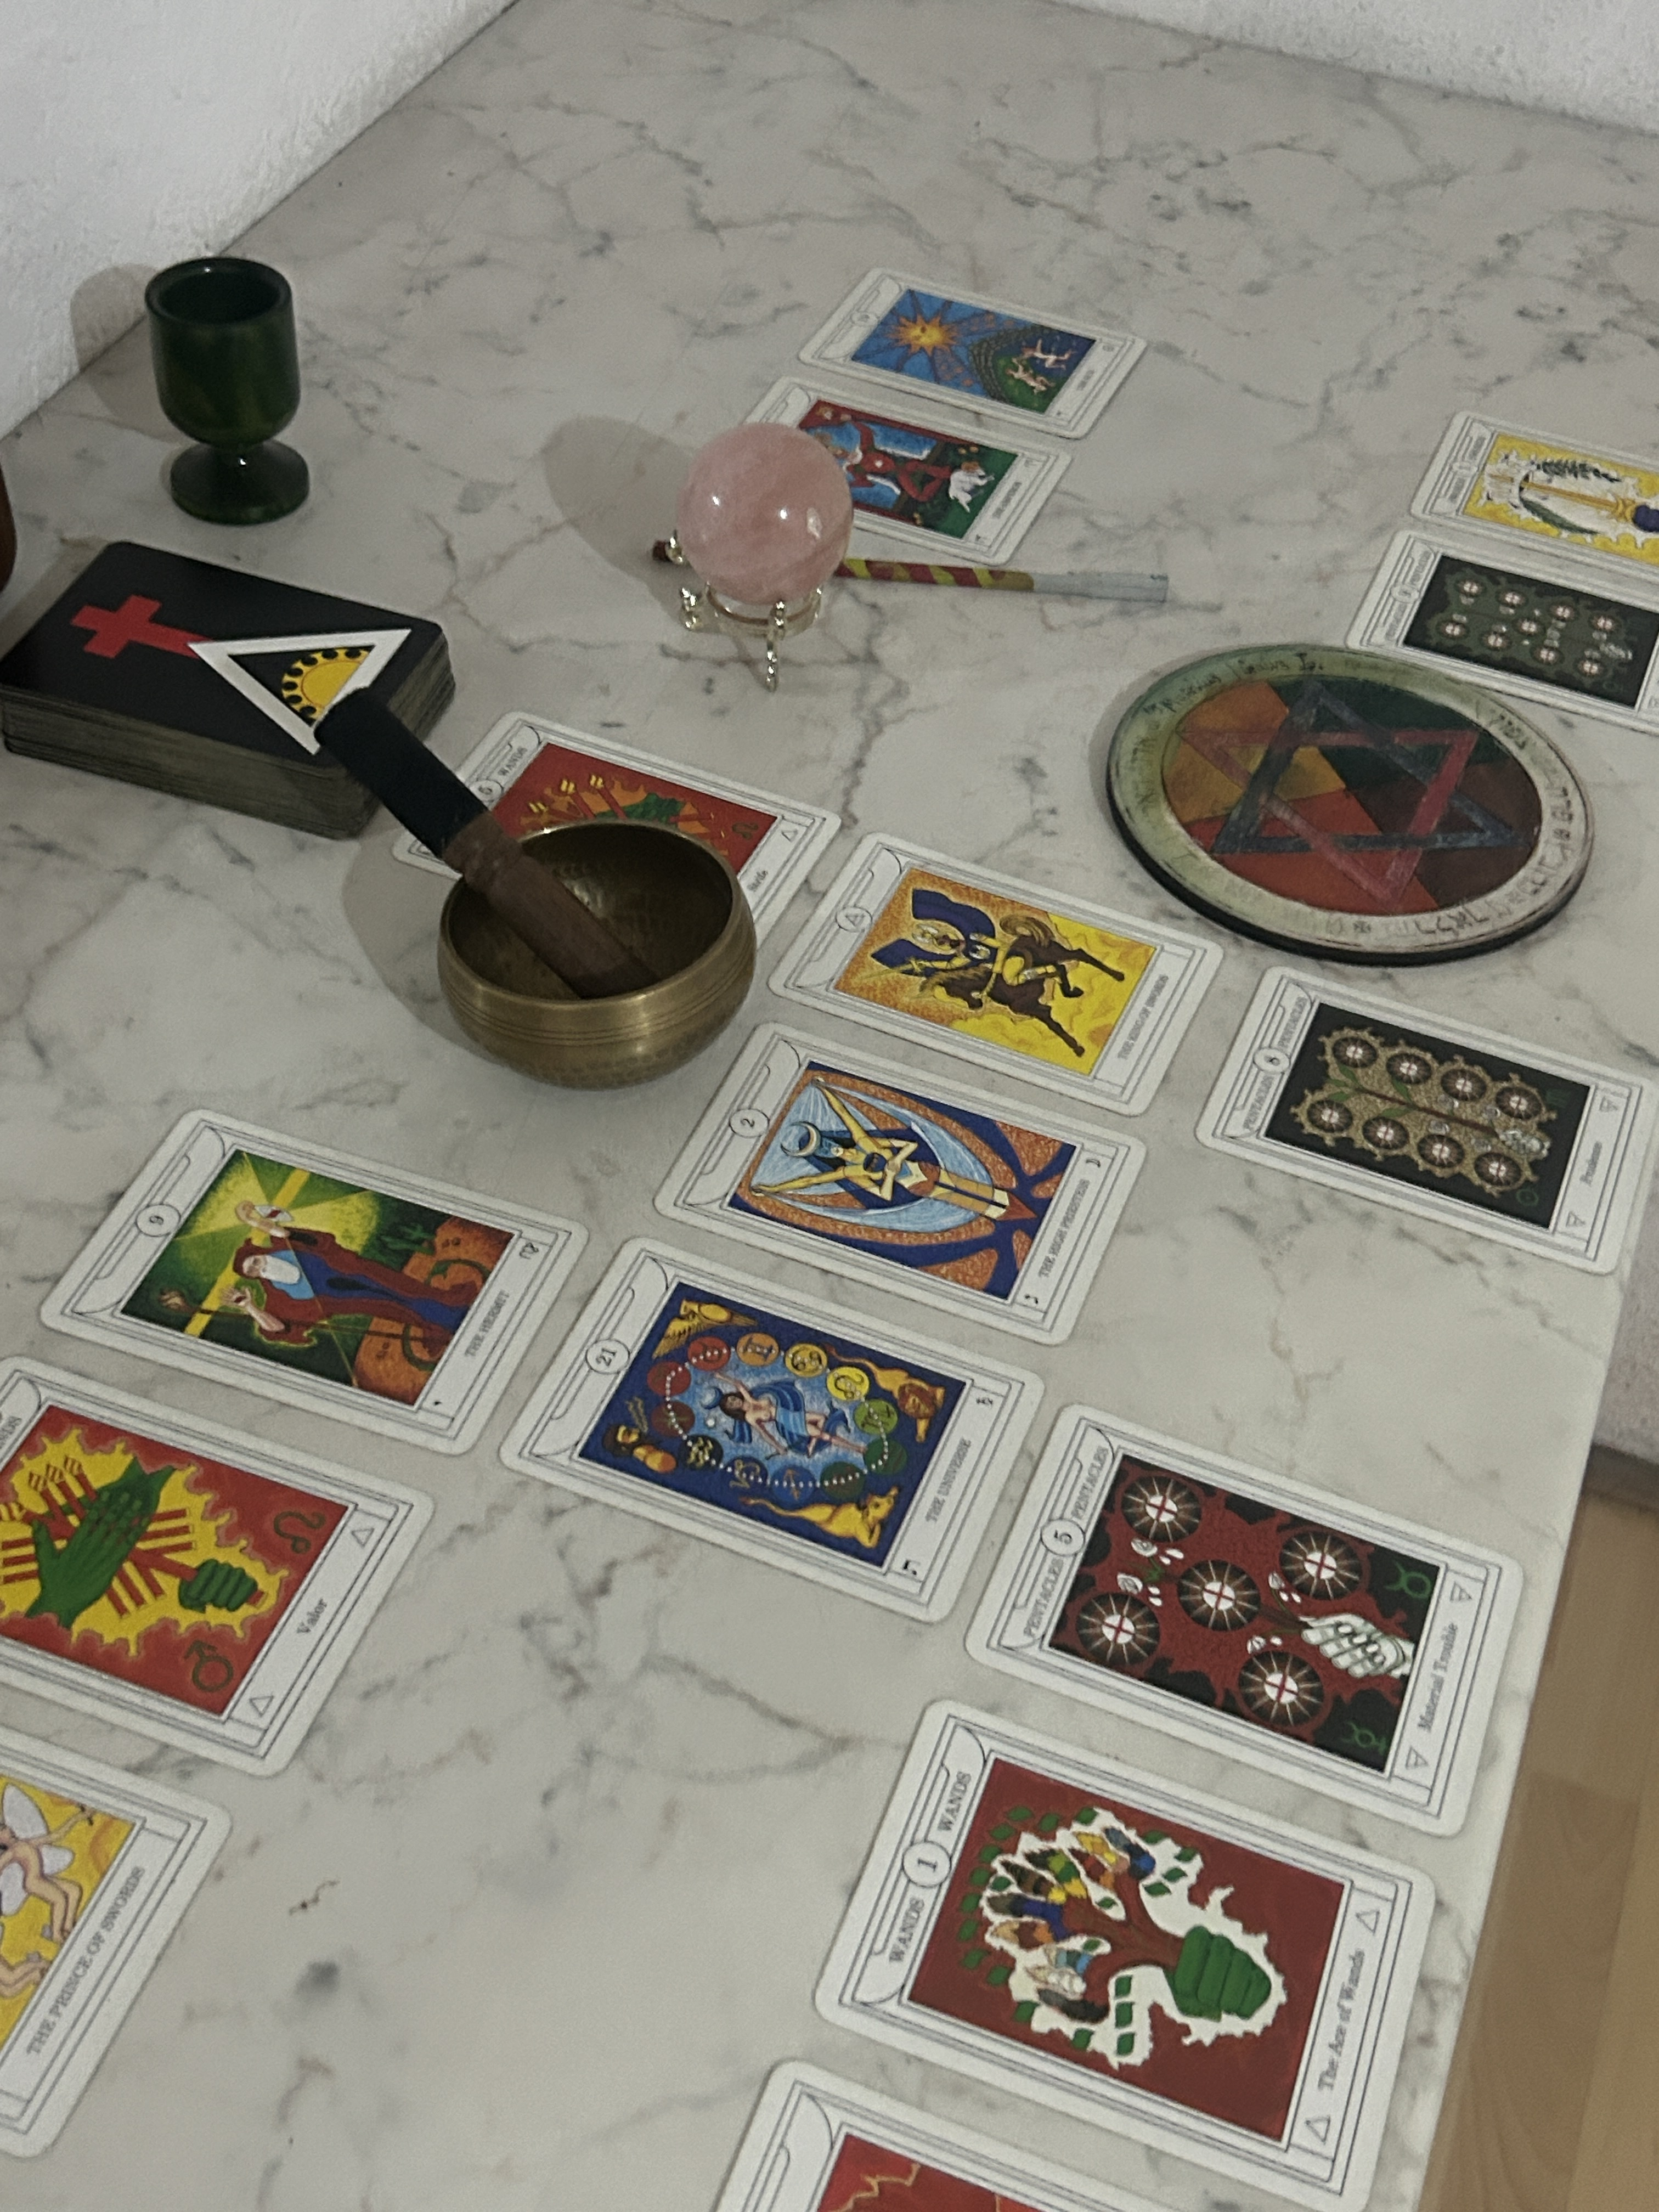
\includegraphics[width=\textwidth,height=\textheight,keepaspectratio]{cover.jpg}
    \vspace*{\fill}
  \end{center}
\end{titlepage}

% ── Title page ───────────────────────────────────────────────────────────────
\begin{titlepage}
  \thispagestyle{empty}
  \begin{center}
    \vspace*{2cm}
    {\Huge\bfseries Cartomantic Practices\\[0.4em]for Practical Use}
    \vspace{2cm}

    \vfill
    {\large 2025}
  \end{center}
\end{titlepage}

\frontmatter
\tableofcontents
\clearpage

% ── Introduction ─────────────────────────────────────────────────────────────
\mainmatter
\chapter*{Introduction}
\addcontentsline{toc}{chapter}{Introduction}
\markboth{Introduction}{Introduction}
\section{Introduction}\label{introduction}

These are working documents, not arguments. Each chapter is a reference for a specific cartomantic instrument --- its structure, its vocabulary, its method. Nothing here requires defense, and none of it needs to be believed in before it can be used.

The question of why divination works is a reasonable one and it has a practical answer that does not require metaphysical commitment. Each system in this book provides a structured symbolic vocabulary --- a finite set of named forces, arranged in a coherent architecture --- and a method for mapping that vocabulary onto a situation. The act of mapping is not passive. It requires the practitioner to select, arrange, and read relationships between symbols, which is another way of saying it requires the practitioner to attend to the situation with a precision that ordinary thinking does not impose. The structure is the value. A good cartomantic system does not tell you what to think --- it tells you what to look at, and in what relationship.

Beyond the structural explanation, each system in this book has an internal logic that amplifies rather than replaces the practitioner\textquotesingle s perception. The Golden Dawn Tarot provides a Qabalistic framework rigorous enough that the card\textquotesingle s meaning is constrained from multiple directions simultaneously --- Sephirah, element, decan, Hebrew letter, and path all converge on a single force, which cannot easily be misread in any of its layers without the other layers correcting it. The Smith-Waite Tarot encodes the same framework beneath pictorial scenes that communicate directly to perception, bypassing the need to consciously calculate correspondences. The Lenormand produces meaning through combination --- single cards are incomplete, and the reader is therefore always working with relationships rather than isolated symbols, which mirrors the relational structure of actual situations. The English playing card system is the most direct of the four: individual cards in positions, read plainly, without cosmological weight.

These are four different instruments for different questions, different registers, and different depths. A complete practice uses the right tool for the right question. The final chapter of this book addresses that question directly.

The chapters run in descending order from the cosmological to the circumstantial: the Golden Dawn Tarot first, the Smith-Waite Tarot second, the English playing card system third, the Lenormand Oracle fourth. There is no required sequence. Each chapter stands alone. The comparison belongs to the final chapter and to the practitioner\textquotesingle s own accumulated experience.

\begin{center}\rule{0.5\linewidth}{0.5pt}\end{center}


% ── Chapter One: Golden Dawn Magical Tarot ───────────────────────────────────
\chapter*{The Golden Dawn Magical Tarot}
\addcontentsline{toc}{chapter}{The Golden Dawn Magical Tarot}
\markboth{The Golden Dawn Magical Tarot}{The Golden Dawn Magical Tarot}
\section{The Demanding Instrument}\label{before-chapter-one-the-golden-dawn-magical-tarot}

We begin with the most demanding instrument because the cosmological framework it establishes underlies everything else in this book. The Golden Dawn Magical Tarot is not merely a divination tool --- it is a complete map of the Western magical tradition rendered in 78 cards. Its Qabalistic structure, its elemental attributions, its astrological correspondences are not decorative. They are the substance. A reader who understands why the Three of Wands is Mars in Aries and what that means on the Tree of Life has access to a precision of interpretation that no amount of intuitive reading can replicate.

This chapter assumes that precision is either already present or being developed alongside the document. What follows is a reference, not a tutorial.

\begin{center}\rule{0.5\linewidth}{0.5pt}\end{center}

\begin{center}\rule{0.5\linewidth}{0.5pt}\end{center}

\clearpage
\input{chapters/golden_dawn_magical_tarot}

% ── Chapter Two: The Smith-Waite Tarot ───────────────────────────────────────
\chapter*{The Smith-Waite Tarot}
\addcontentsline{toc}{chapter}{The Smith-Waite Tarot}
\markboth{The Smith-Waite Tarot}{The Smith-Waite Tarot}
\input{chapters/preface_sw}
\clearpage
\chapter{The Smith-Waite Tarot}\label{the-smith-waite-tarot}

\section{Operating Principles}\label{operating-principles}

The Smith-Waite Tarot was designed by Pamela Colman Smith under the direction of Arthur Edward Waite, completed in 1909 in Smith\textquotesingle s Chelsea studio. Smith painted all 78 images in six months using ink and watercolor, working from Waite\textquotesingle s detailed instructions for the Major Arcana and from her own invention for the Minor Arcana pip cards. The pictorial scenes on the 56 Minor Arcana cards --- the single most significant development in tarot history --- were Smith\textquotesingle s creation, not Waite\textquotesingle s. Waite had little interest in the Minors. Smith transformed what had been geometric arrangements of suit symbols into a complete visual vocabulary for human experience.

Both were members of the Hermetic Order of the Golden Dawn. The esoteric framework of the deck is therefore the same Qabalistic structure underlying the Golden Dawn Magical Tarot --- Hebrew letters, Paths on the Tree of Life, elemental and astrological correspondences. Waite deliberately obscured some of this structure for non-initiates while retaining it intact beneath the surface. The deck was designed to function both as a divinatory tool for general use and as an esoteric instrument for those with the training to read its deeper layers. It succeeds at both simultaneously.

Smith\textquotesingle s monogram --- a serpentine snake entwined around her initials --- appears on every card. It is the only authorial mark on the deck and she placed it there herself.

This system uses reversals. An upright card and a reversed card carry different meanings. This distinguishes it from both the Golden Dawn system (which uses elemental dignities) and the English playing card system (which uses position and combination).

\begin{center}\rule{0.5\linewidth}{0.5pt}\end{center}

\section{The Structure}\label{the-structure}

78 cards in two groups:

\textbf{The Major Arcana} --- 22 keys numbered 0 through XXI. These follow the Golden Dawn Path structure: each key is a Path on the Tree of Life connecting two Sephiroth, carrying a Hebrew letter, an astrological attribution, and a specific force. Waite retained the GD framework but corrected one significant misalignment in the original Book T correspondence (see Departures section).

\textbf{The Minor Arcana} --- 56 cards in four suits of 14 cards each: Ace through 10, plus four court cards (King, Queen, Knight, Page). The 40 pip cards (Ace through 10) carry Smith\textquotesingle s pictorial scenes. The 16 court cards carry armored or robed figures whose expression, posture, and environment Smith used to convey character rather than merely rank.

\begin{center}\rule{0.5\linewidth}{0.5pt}\end{center}

\section{The Suits and Their Correspondences}\label{the-suits-and-their-correspondences}

\textbf{Wands --- Fire} Will, enterprise, ambition, the creative and spiritual impulse, energy before it finds form. The suit of what is being initiated or driven forward. Wands figures are generally depicted in landscapes of open sky and bare hills --- the unformed territory that fire moves through.

\textbf{Cups --- Water} Emotion, imagination, the interior life, relationship, the unconscious. The suit of feeling and vision. Cup scenes often feature water, calm or turbulent, and emphasize interiority --- figures contemplating, dreaming, receiving.

\textbf{Swords --- Air} Intellect, conflict, truth, the consequence of thought and word. The most difficult suit in the deck. Swords scenes frequently depict aftermath --- the storm has passed or is passing, figures standing in the wreckage of what clear thought or harsh truth has produced. Air both clarifies and cuts.

\textbf{Pentacles --- Earth} The material world, the body, money, craft, the practical result. The suit of what has actually manifested. Pentacle scenes tend toward ordered gardens, cultivated land, workshops --- the world where human effort meets physical reality.

\begin{center}\rule{0.5\linewidth}{0.5pt}\end{center}

\section{The Esoteric Framework}\label{the-esoteric-framework}

Waite retained the Golden Dawn Qabalistic structure beneath the surface of the deck. The 22 Major Arcana correspond to the 22 Paths on the Tree of Life. The 10 pip numbers per suit correspond to the 10 Sephiroth. The four suits correspond to the four worlds (Atziluth, Briah, Yetzirah, Assiah) and to the four letters of YHVH.

This framework is not printed on the cards and Waite deliberately withheld the correspondences from his written commentary to protect initiatory teaching from general publication. The Pictorial Key to the Tarot (1910), his companion volume, is notably evasive on these points while accurate on divinatory meanings. The full correspondence system must be drawn from the Golden Dawn documents directly.

For practical reference, the Sephirothic assignments of the pip cards are identical to those in the Golden Dawn system:

\begin{longtable}[]{@{}>{\RaggedRight\small}p{0.18\linewidth}>{\RaggedRight\small}p{0.22\linewidth}>{\RaggedRight\small}p{0.54\linewidth}@{}}
\toprule\noalign{}
Number & Sephirah & Character \\
\midrule\noalign{}
\endhead
\bottomrule\noalign{}
\endlastfoot
Ace & Kether & Root force; undivided, radical power of the suit \\
2 & Chokmah & Initial polarity; the first differentiation; beginnings \\
3 & Binah & First concrete form; realization through limitation \\
4 & Chesed & Stability; the foundation established \\
5 & Geburah & Disruption; the established order disturbed \\
6 & Tiphareth & Harmony; accomplished success; the solar center \\
7 & Netzach & Force seeking outlet; result dependent on action \\
8 & Hod & Swift directed force; precise but potentially hasty \\
9 & Yesod & Fundamental strength; the approach of completion \\
10 & Malkuth & Final manifestation; the matter fully determined \\
\end{longtable}

\begin{center}\rule{0.5\linewidth}{0.5pt}\end{center}

\section{Key Departures from the Golden Dawn Tradition}\label{key-departures-from-the-golden-dawn-tradition}

\textbf{The Strength/Justice correction.} In the original Golden Dawn Book T, the astrological correspondence assigned Leo (Teth) to Key VIII and Libra (Lamed) to Key XI. In the traditional Marseilles ordering, Key VIII is Justice and Key XI is Strength. This produced a mismatch: the Justice card (scales imagery) was assigned to Leo, and the Strength card (lion imagery) was assigned to Libra --- the reverse of what the iconography implies.

Waite corrected this by swapping the two cards:

\begin{itemize}
\tightlist
\item
  Key VIII = \textbf{Strength} = Teth = Leo (lion imagery now matches Leo attribution)
\item
  Key XI = \textbf{Justice} = Lamed = Libra (scales imagery now matches Libra attribution)
\end{itemize}

This swap is the most significant structural departure from both the Marseilles tradition and from the original GD numbering. The Golden Dawn Magical Tarot (Cicero) follows the same corrected order.

The Marseilles tradition: Justice = VIII, Strength = XI. Smith-Waite and Cicero GD: Strength = VIII, Justice = XI.

When working across decks, this is the single most important structural difference to track.

\textbf{The pictorial Minor Arcana.} All tarot decks before Smith-Waite used geometric arrangements of suit symbols for the pip cards --- four cups arranged in a pattern for the Four of Cups, eight swords for the Eight of Swords. There were no narrative scenes. Smith introduced pictorial scenes to all 40 pip cards (Ace through Ten in each suit). These scenes were her invention, developed from Waite\textquotesingle s suit meanings with considerable creative latitude. The Minor Arcana as a pictorial narrative vocabulary is Smith\textquotesingle s contribution to the tradition, not Waite\textquotesingle s.

The consequence for reading practice is significant: Smith\textquotesingle s scenes communicate meaning directly through image, bypassing the need to know the underlying Qabalistic or astrological structure. A reader who knows nothing of Sephiroth can read the Five of Swords (three figures, two retreating in defeat, one gathering the swords with a cold expression) and derive its meaning accurately from the scene alone. This is what made the deck accessible to non-initiates and what drove its dominance throughout the twentieth century.

\textbf{Court card naming.} Waite reverted to traditional pre-GD naming for the court cards: King, Queen, Knight, Page. The GD used King, Queen, Prince, Princess to reflect the YHVH tetrad (Yod, Heh, Vau, Heh final). Waite\textquotesingle s naming obscures the elemental-rank correspondence:

\begin{itemize}
\tightlist
\item
  Smith-Waite \textbf{Knight} (mounted) corresponds to GD \textbf{King} (Yod, Fire of the suit)
\item
  Smith-Waite \textbf{King} (seated) corresponds to GD \textbf{Prince} (Vau, Air of the suit)
\item
  Smith-Waite \textbf{Queen} = GD \textbf{Queen} (Heh, Water of the suit)
\item
  Smith-Waite \textbf{Page} = GD \textbf{Princess} (Heh final, Earth of the suit)
\end{itemize}

This means the most senior court card by elemental rank in the GD system --- the Yod, Fire quality --- is called the Knight in Smith-Waite, while the card called King is actually the third in elemental seniority. Waite did not document this alignment clearly and modern readers largely ignore it, reading the courts by scene and character rather than elemental rank.

\textbf{Renaming of Major Arcana.} Waite renamed several cards from their traditional titles: the Papess became the High Priestess, the Pope became the Hierophant. These renamings removed Catholic imagery in favor of broader esoteric terminology consistent with the GD\textquotesingle s non-denominational magical framework.

\begin{center}\rule{0.5\linewidth}{0.5pt}\end{center}

\section{The Major Arcana}\label{the-major-arcana}

\begin{longtable}[]{@{}>{\RaggedRight\small}p{0.08\linewidth}>{\RaggedRight\small}p{0.12\linewidth}>{\RaggedRight\small}p{0.10\linewidth}>{\RaggedRight\small}p{0.10\linewidth}>{\RaggedRight\small}p{0.12\linewidth}>{\RaggedRight\small}p{0.42\linewidth}@{}}
\toprule\noalign{}
Key & Name & Hebrew Letter & Attribution & Path & Waite\textquotesingle s Title \\
\midrule\noalign{}
\endhead
\bottomrule\noalign{}
\endlastfoot
0 & The Fool & Aleph & Air & 11 (Kether--Chokmah) & Spirit of the Ether \\
I & The Magician & Beth & Mercury & 12 (Kether--Binah) & Magus of Power \\
II & The High Priestess & Gimel & Moon & 13 (Kether--Tiphareth) & Priestess of the Silver Star \\
III & The Empress & Daleth & Venus & 14 (Chokmah--Binah) & Daughter of the Mighty Ones \\
IV & The Emperor & Heh & Aries & 15 (Chokmah--Tiphareth) & Son of the Morning \\
V & The Hierophant & Vau & Taurus & 16 (Chokmah--Chesed) & Magus of the Eternal \\
VI & The Lovers & Zayin & Gemini & 17 (Binah--Tiphareth) & Children of the Voice \\
VII & The Chariot & Cheth & Cancer & 18 (Binah--Geburah) & Child of the Powers of the Waters \\
VIII & Strength & Teth & Leo & 19 (Chesed--Geburah) & Daughter of the Flaming Sword \\
IX & The Hermit & Yod & Virgo & 20 (Chesed--Tiphareth) & Prophet of the Eternal \\
X & Wheel of Fortune & Kaph & Jupiter & 21 (Chesed--Netzach) & Lord of the Forces of Life \\
XI & Justice & Lamed & Libra & 22 (Geburah--Tiphareth) & Daughter of the Lords of Truth \\
XII & The Hanged Man & Mem & Water & 23 (Geburah--Hod) & Spirit of the Mighty Waters \\
XIII & Death & Nun & Scorpio & 24 (Tiphareth--Netzach) & Child of the Great Transformers \\
XIV & Temperance & Samekh & Sagittarius & 25 (Tiphareth--Yesod) & Daughter of the Reconcilers \\
XV & The Devil & Ayin & Capricorn & 26 (Tiphareth--Hod) & Lord of the Gates of Matter \\
XVI & The Tower & Peh & Mars & 27 (Netzach--Hod) & Lord of the Hosts of the Mighty \\
XVII & The Star & Tzaddi & Aquarius & 28 (Netzach--Yesod) & Daughter of the Firmament \\
XVIII & The Moon & Qoph & Pisces & 29 (Netzach--Malkuth) & Ruler of Flux and Reflux \\
XIX & The Sun & Resh & Sol & 30 (Hod--Yesod) & Lord of the Fire of the World \\
XX & Judgement & Shin & Fire & 31 (Hod--Malkuth) & Spirit of the Primal Fire \\
XXI & The World & Tau & Saturn & 32 (Yesod--Malkuth) & Great One of the Night of Time \\
\end{longtable}

\subsection{Major Arcana: Smith\textquotesingle s Scenes and Waite\textquotesingle s Meanings}\label{major-arcana-smiths-scenes-and-waites-meanings}

\textbf{0 --- The Fool} \emph{Scene:} A young figure in ornate clothing steps toward the edge of a cliff, eyes upward, carrying a white rose and a small pack on a wand. A small dog leaps at his heels. Mountains behind. Sky clear. \emph{Upright:} Folly, mania, extravagance in the best sense --- the leap into the unknown that is also pure spiritual potential. The beginning before beginning. Unconditioned. \emph{Reversed:} Negligence, apathy, the leap made without attention; foolishness without redemption.

\textbf{I --- The Magician} \emph{Scene:} A figure in red and white robes stands before a table bearing the four suit symbols. One hand raises a wand toward heaven; one points to earth. Above his head, the lemniscate (infinity sign). About his waist, a serpent devouring its own tail. \emph{Upright:} Skill, will, self-confidence, the capacity to act. The directed use of all available resources. Initiation of a new cycle. \emph{Reversed:} Will misdirected; skill used for manipulation; the appearance of power without its substance.

\textbf{II --- The High Priestess} \emph{Scene:} A crowned figure sits between two pillars --- one black (Boaz), one white (Jachin) --- before a veil hung with pomegranates. A crescent moon at her feet. She holds a scroll marked TORA, partially concealed. \emph{Upright:} Hidden knowledge, the unconscious, what is not yet revealed, inner wisdom accessible only through stillness. The unrealized future. \emph{Reversed:} Superficial knowledge; what is hidden used for manipulation; passion overriding wisdom.

\textbf{III --- The Empress} \emph{Scene:} A crowned, pregnant figure sits in a field of ripe grain before a forest. Heart-shaped shield bearing the Venus symbol. Flowing robes covered in pomegranates. \emph{Upright:} Fertility, abundance, nature, the creative force in full productive expression. Growth, sensory pleasure, domestic life flourishing. \emph{Reversed:} Inaction, dissipation, creative energy without outlet or squandered.

\textbf{IV --- The Emperor} \emph{Scene:} An armored, bearded figure sits rigidly on a stone throne decorated with rams\textquotesingle{} heads. He holds an ankh and an orb. Mountains behind --- hard and red. \emph{Upright:} Temporal power, governance, the establishing of order through will and force. Authority, the father. Dominion over the material world. \emph{Reversed:} Domination, rigidity, the abuse of authority; weakness concealed behind show of force.

\textbf{V --- The Hierophant} \emph{Scene:} A robed, crowned figure sits between two pillars, right hand raised in blessing. Two supplicants kneel before him. Two crossed keys at his feet. \emph{Upright:} Established institutions and their wisdom, teaching, the transmission of sacred knowledge, religious or formal initiation. The outer form of inner truth. \emph{Reversed:} Dogma mistaken for wisdom; conformity; the institution protecting itself rather than serving.

\textbf{VI --- The Lovers} \emph{Scene:} A man and woman stand naked before an angel in the sky --- Adam and Eve before the angel Raphael. Behind the woman, the Tree of Knowledge. Behind the man, a tree of flame. Mountain in the distance. \emph{Upright:} The right choice made through love and aspiration rather than calculation. Union, harmony, alignment of values. The beginning of genuine partnership. \emph{Reversed:} Wrong choice; separation; values in conflict with each other.

\textbf{VII --- The Chariot} \emph{Scene:} A crowned warrior stands in a stone chariot drawn by two sphinxes --- one black, one white --- in apparent opposition. He carries a wand and is armored. Stars above, city behind. \emph{Upright:} Triumph through the mastery of opposing forces. Victory, discipline, the will directing contradictory energies toward a single end. Conquest. \emph{Reversed:} Defeat by one\textquotesingle s own contradictions; victory sought without ethical grounding.

\textbf{VIII --- Strength} \emph{Scene:} A woman in white, crowned with flowers, gently closes the mouth of a lion. The lemniscate above her head. No struggle --- she holds the beast with ease. \emph{Upright:} Courage, patience, the gentle mastery of one\textquotesingle s own animal nature. Force that does not need violence. Endurance. The strength that comes from inner certainty. \emph{Reversed:} Weakness, abuse of power, desire overriding judgment.

\textbf{IX --- The Hermit} \emph{Scene:} An old, robed figure stands alone on a snowy peak. He holds a lantern containing a six-pointed star --- the Seal of Solomon. He carries a staff. \emph{Upright:} Wisdom sought and found in solitude. The guide who has completed the journey and now carries the light for others. Prudence. Withdrawal in service of illumination. \emph{Reversed:} Excessive withdrawal, fear disguised as wisdom; refusing the return.

\textbf{X --- Wheel of Fortune} \emph{Scene:} A large wheel inscribed with alchemical and Qabalistic symbols turns in space. A sphinx sits on top; below, Typhon descends. Four winged figures at the corners hold books --- the symbols of the four fixed signs (man, eagle, lion, bull). \emph{Upright:} Fortune turning, good luck arriving, the completion of a cycle. What rises when the wheel moves. The larger pattern asserting itself. \emph{Reversed:} Fortune turning downward; bad luck; resistance to necessary change.

\textbf{XI --- Justice} \emph{Scene:} A crowned, robed figure sits between two pillars, holding scales in one hand and an upraised sword in the other. The figure is still, formal, impartial. \emph{Upright:} Equity, righteous judgment, the truth of the situation as it actually stands. What is fair. Legal matters decided correctly. The equilibrating principle. \emph{Reversed:} Bias, legal injustice, judgment corrupted by interest.

\textbf{XII --- The Hanged Man} \emph{Scene:} A young man hangs by one foot from a T-shaped wooden frame between two living trees. His expression is calm, almost radiant. A halo of light surrounds his head. His free leg crosses behind the suspended leg, forming a figure four. \emph{Upright:} Willing sacrifice, suspension, the reversal of ordinary values that allows a higher perspective. What cannot be forced. The necessary pause. \emph{Reversed:} Arrogance in sacrifice; the martyrdom that serves the ego; wasted sacrifice.

\textbf{XIII --- Death} \emph{Scene:} An armored skeleton on a white horse moves through a field. A king lies dead before it. A bishop approaches in prayer. A young woman turns away. A child offers flowers. In the distance, the sun rises between two towers. \emph{Upright:} Transformation, the necessary end. What must die for what is next to begin. The card rarely means physical death --- it means the death of a situation, identity, or phase of life. \emph{Reversed:} Stagnation, the refusal to let something die that has finished; inertia.

\textbf{XIV --- Temperance} \emph{Scene:} An angel stands with one foot on land, one in water, pouring liquid between two cups in a continuous stream. Irises grow near the water. A path leads toward mountains and a shining crown in the sky. \emph{Upright:} The combination of forces into a working whole. Moderation as an active art. The alchemical mixing that produces something neither ingredient contained. Patience, adaptation, balance in motion. \emph{Reversed:} Discord, competing forces that will not combine; excess.

\textbf{XV --- The Devil} \emph{Scene:} A goat-headed figure sits on a black cube to which two human figures are chained by loose chains --- they could remove them. The figures have horns and tails. The Devil holds an inverted torch. \emph{Upright:} Bondage to the material plane, to habit, to compulsion. The chains are chosen, not locked. The force of matter fully realized --- which may serve or bind depending on how it is engaged. \emph{Reversed:} Beginning of release from bondage; the first recognition of the chain.

\textbf{XVI --- The Tower} \emph{Scene:} Lightning strikes a tall stone tower. A crown is blasted from its top. Two figures fall headlong. Flames issue from the windows. \emph{Upright:} Sudden catastrophic change. The structure built on false foundations is struck down. Cannot be avoided once in motion. Sometimes liberation through destruction. \emph{Reversed:} The catastrophe suppressed, postponed, built up further; oppression.

\textbf{XVII --- The Star} \emph{Scene:} A naked woman kneels at the edge of water, pouring from two vessels --- one into the water, one onto the land. Eight stars above her, one large and central. \emph{Upright:} Hope, faith, spiritual nourishment freely given. The grace that arrives after the darkness of The Tower. Clarity, inspiration, unexpected help. \emph{Reversed:} Hope deferred; self-doubt masquerading as realism; gifts withheld.

\textbf{XVIII --- The Moon} \emph{Scene:} A full moon with a face looks down on two towers. A wolf and a dog howl at it from either side of a path that leads into the distance. A crayfish emerges from a pool. \emph{Upright:} Illusion, deception, the terror and fertility of the unconscious. The liminal state between worlds. Things are not as they appear. The path must be walked without full sight. \emph{Reversed:} Deception recognized too late; practical mistakes; confusion less than feared.

\textbf{XIX --- The Sun} \emph{Scene:} A large radiant sun shines down on a naked child riding a white horse before a wall hung with sunflowers. The child holds a red banner. \emph{Upright:} Success, contentment, clarity, the pleasure of being fully alive in a good world. The most unambiguously fortunate of the Major Arcana. \emph{Reversed:} Success delayed or diminished; happiness present but obscured.

\textbf{XX --- Judgement} \emph{Scene:} An angel blows a trumpet from the clouds. Figures rise from coffins below --- men, women, children --- with arms raised. A mountain range in the distance. \emph{Upright:} The call that cannot be ignored. The final reckoning with one\textquotesingle s own past. A decisive outcome. The awakening to what one has actually been. \emph{Reversed:} The call heard but refused; delay in reckoning; the awakening postponed.

\textbf{XXI --- The World} \emph{Scene:} A naked figure dances within a laurel wreath, holding two wands. Four winged figures at the corners --- bull, lion, eagle, angel --- the fixed signs. The wreath is oval, enclosing the dancer completely. \emph{Upright:} Synthesis, completion, the successful conclusion of a long cycle. The world as it actually is --- whole. Often describes the situation itself rather than adding a force to it. \emph{Reversed:} Incomplete success; the final step not yet taken; stagnation at the threshold of completion.

\begin{center}\rule{0.5\linewidth}{0.5pt}\end{center}

\section{The Aces}\label{the-aces}

The Aces are Kether of their suit --- the root force before it differentiates into the ten Sephiroth below. In Smith\textquotesingle s images, each Ace presents a single hand emerging from a cloud, offering the suit symbol. The hand is the hand of the divine --- impersonal, neither male nor female, offering the instrument to whoever will take it.

\textbf{Ace of Wands} A hand offers a single flowering wand. Flames leave its tip. A castle in the distance. \emph{Upright:} The beginning of a creative or spiritual enterprise. Raw initiative. The spark that precedes the fire. Fortune and enterprise. \emph{Reversed:} Delays in starting; false start; the initiative that collapses before it builds.

\textbf{Ace of Cups} A chalice overflows into a pool below. A dove descends with a communion wafer. The cup has five streams pouring from it. \emph{Upright:} The beginning of love, abundance, joy, spiritual nourishment freely offered. The overflowing source. A new emotional beginning. \emph{Reversed:} Love withdrawn; the cup offered but refused; spiritual emptiness.

\textbf{Ace of Swords} A hand holds a sword upright, crowned at its tip. Mountains below, barren. The crown is circled with the wreath of victory, trailing olive and palm. \emph{Upright:} The invoked power of the mind --- clarity, triumph, the force of truth. When raised toward heaven, the sword calls down divine clarity. The double edge: the same force liberates or destroys depending on how it is held. \emph{Reversed:} The blade turned against its bearer. Tyranny, disaster, the force of intellect misused.

\textbf{Ace of Pentacles} A hand offers a single large pentacle against a garden of white lilies and roses. A gate leads through a hedge into a mountainous distance. \emph{Upright:} Material prosperity, the beginning of a practical achievement, the seed of physical manifestation. The gate to the material garden is open. \emph{Reversed:} Prosperity blocked or misused; material opportunity refused.

\begin{center}\rule{0.5\linewidth}{0.5pt}\end{center}

\section{The Court Cards}\label{the-court-cards}

Court cards represent people in the querent\textquotesingle s life, the querent in a particular mode, or dominant forces shaping the situation. Smith gave each court figure a specific environment, expression, and posture that communicates character directly. The elemental assignments follow the same logic as the Golden Dawn system --- see the Departures section for the naming correspondence.

\subsection{Kings --- Seated figures; established authority; the mature expression of the suit\textquotesingle s force}\label{kings--seated-figures-established-authority-the-mature-expression-of-the-suits-force}

\textbf{King of Wands} Enthroned in the open air, armored, holding a flowering wand. Salamanders on his robe. A lion on the throne. He leans forward slightly --- alert, not resting. A generous, fiery, noble person. Quick in action and affection, impulsive, passionate. Natural authority that burns fast and moves on. \emph{Reversed:} Severity, prejudice, or the fire turned to arrogance.

\textbf{King of Cups} Enthroned on a stone block in the middle of a turbulent sea. He holds a cup and a short scepter. A fish leaps from the sea behind him. He appears calm amid the storm. A man of feeling who has mastered his interior life --- creative, skilled, emotionally intelligent. Commands without suppression. \emph{Reversed:} Craftiness and unscrupulousness; emotional manipulation.

\textbf{King of Swords} Enthroned, facing forward, armored, sword raised. His throne is decorated with butterflies and sylphs. The sky behind him is overcast with wind-bent trees. A figure of keen intellect and authority. Analytical, decisive, active in matters requiring judgment. Can be severe, even ruthless when convinced of being right. \emph{Reversed:} Cruelty, perversity, deliberate harm.

\textbf{King of Pentacles} Enthroned in a garden. His robe is covered with grapes and flowers. His throne is decorated with bulls\textquotesingle{} heads. He holds a pentacle and a scepter. Reliable, established, successful in material domains. Patient, methodical, not easily moved. His wealth is earned and maintained rather than won. The steward. \emph{Reversed:} Vice, weakness, corruption of what was solid.

\subsection{Queens --- Seated figures; receptive, interior power; the suit\textquotesingle s force made stable}\label{queens--seated-figures-receptive-interior-power-the-suits-force-made-stable}

\textbf{Queen of Wands} Enthroned before sunflowers. She holds a sunflower in one hand, a wand in the other. A black cat sits at her feet. She faces outward --- open, confident. Practical and fiery. Self-directed, passionate, attractive in personality. Loyal when her loyalty is earned. The most independent of the queens. \emph{Reversed:} Jealousy, fickleness, opposition wearing a friendly face.

\textbf{Queen of Cups} Enthroned at the water\textquotesingle s edge, holding an elaborate closed cup that she contemplates. Her robe flows into the sea. She does not look at the observer. Profoundly intuitive, visionary, emotionally deep. A person who receives impressions from the unconscious and can communicate them. The interior life is her home. \emph{Reversed:} The same depths become perversity; the vision turns to delusion.

\textbf{Queen of Swords} Enthroned on a cloud-height throne. Sword raised, left hand extended as if beckoning. Her expression is stern but not unkind. Sylphs in the clouds around her. A person who has experienced loss and sees clearly as a result. Keen, just, quick in perception. May have suffered, but the suffering has produced precision rather than bitterness. \emph{Reversed:} Malice, narrow-mindedness; sorrow used as a weapon.

\textbf{Queen of Pentacles} Enthroned in a garden surrounded by flowers and fruit. A rabbit runs at the lower corner. She holds a pentacle and contemplates it with gentleness. Practical, nurturing, resourceful. The ability to make any environment fertile. Generous with what she has. Entirely at home in the physical world. \emph{Reversed:} Neglect of the domestic world; suspicion; materialism without generosity.

\subsection{Knights --- Mounted figures; active, initiating force; the suit in motion}\label{knights--mounted-figures-active-initiating-force-the-suit-in-motion}

\textbf{Knight of Wands} On a rearing horse in an arid landscape, armored in red and gold with salamanders on his tunic. He charges forward, wand raised. Energetic, impulsive, departure from what is familiar, travel, a sudden journey. The fire force in full movement --- brilliant and unreliable by turns. \emph{Reversed:} Interruption, discord, the charge that leads nowhere.

\textbf{Knight of Cups} On a slow-walking horse in a calm landscape, armored, holding a cup forward as if presenting it. Wings on his helmet. River and fish in the distance. A romantic approach, an invitation, a proposition. Someone who brings feeling forward rather than acting immediately. The arrival of a love interest or a creative offer. \emph{Reversed:} Fraud, trickery; the romantic gesture that conceals manipulation.

\textbf{Knight of Swords} On a charging horse, armor flying, sword raised. The sky behind him is turbulent, trees bent by wind. He moves with absolute speed and commitment. Forceful, brave, domineering, impulsive in the extreme. The mind in full charge. Can be heroic or catastrophically ill-timed depending on circumstances. \emph{Reversed:} Imprudence, extravagance, the charge that destroys everything including the purpose it was meant to serve.

\textbf{Knight of Pentacles} On a stationary heavy horse in a plowed field. He holds a pentacle and studies it. Armored in dull greens and browns. Nothing is moving. Responsible, patient, methodical, dependable to the point of immobility. The person who will actually complete the task correctly and without drama. \emph{Reversed:} Stagnation, idleness, materialism as an end in itself.

\subsection{Pages --- Standing figures; nascent energy; new beginnings and messages}\label{pages--standing-figures-nascent-energy-new-beginnings-and-messages}

\textbf{Page of Wands} Stands in an arid landscape holding a long wand, looking at it with curiosity. His cap has a feather. Young, attentive, fired with new possibility. A bearer of news, a faithful young person, a creative impulse not yet in motion. Something is about to begin; the messenger has arrived. \emph{Reversed:} Bad news; an unstable young person; a project that will not begin.

\textbf{Page of Cups} Stands at the water\textquotesingle s edge holding a cup from which a fish has emerged and appears to be speaking to him. He regards it with gentle surprise. Reflective news, a message with emotional content. A gentle, dreamy young person or the beginning of an imaginative project. The unexpected that arrives from the interior. \emph{Reversed:} Deception, seduction; the dream that misleads.

\textbf{Page of Swords} Stands on a windswept cliff, sword raised, looking alertly about. His posture is ready, slightly suspicious. Vigilance, insight, the need to be alert. A perceptive young person. News involving scrutiny or negotiation. The arrival of a situation requiring sharp attention. \emph{Reversed:} The same vigilance turned to cunning or spying.

\textbf{Page of Pentacles} Stands in a garden holding a pentacle up before him and gazing at it with concentration. Flowers at his feet. Young, serious, absorbed. Practical news, the beginning of a material project, a diligent young person with capacity for growth. Scholarship or apprenticeship. \emph{Reversed:} Dissipation, wastefulness, the practical gift squandered.

\begin{center}\rule{0.5\linewidth}{0.5pt}\end{center}

\section{The Minor Arcana: Pip Cards 2--10}\label{the-minor-arcana-pip-cards-210}

Smith\textquotesingle s scenes are not arbitrary decoration --- they are pictorial statements of the card\textquotesingle s force, derived from the Sephirothic and astrological attributions underlying each card. Reading the scene is reading the force. The upright meaning follows the scene\textquotesingle s narrative; the reversed meaning is generally the same force turned inward, blocked, or distorted.

\subsection{Wands}\label{wands}

\begin{longtable}[]{@{}>{\RaggedRight\small}p{0.14\linewidth}>{\RaggedRight\small}p{0.18\linewidth}>{\RaggedRight\small}p{0.20\linewidth}>{\RaggedRight\small}p{0.42\linewidth}@{}}
\toprule\noalign{}
Card & Smith\textquotesingle s Scene & Upright & Reversed \\
\midrule\noalign{}
\endhead
\bottomrule\noalign{}
\endlastfoot
2 & A figure on a castle wall holds a globe, gazing at the sea. A second wand is fixed beside him. & Will established, planning the next step from a position of strength. Personal power, boldness. & Surprise, fear of the unknown, anticipation turning to anxiety. \\
3 & A figure with his back to us watches ships depart from a high place. Three wands are planted. & Enterprise under way. Practical success. The work in motion, the ships launched. & Caution, disappointment, beware of pride. \\
4 & Garlands hang between four wands. Two figures approach in celebration. A castle behind. & Completion, harvest, the rest that follows genuine effort. Prosperity, harmony, a settled situation. & Prosperity and happiness not fully claimed; beauty and completion withheld slightly. \\
5 & Five figures in open conflict, each wielding a wand against the others. & Strife, competition, conflict of interests. Not catastrophe --- the friction of opposed wills. & Contradiction, litigation, disputes. \\
6 & A mounted figure in laurel crown moves through a crowd, wand held high. Others hold wands alongside. & Victory, public recognition, good news. The successful outcome of a contest. & Apprehension of failure, disloyalty, the crown not yet secure. \\
7 & A figure defends a high position against six wands rising from below. & Valor, the courage to hold a position against opposition. Advantage from strength. & Perplexity, anxiety, embarrassment, being overwhelmed. \\
8 & Eight wands fly through open air over a landscape --- in transit, pointing toward a landing. & Movement, swift action, things arriving. News in transit. Haste. & Arrows of jealousy, quarrels, delays. \\
9 & A battered figure leans on a wand, guarding a row of eight behind him. He looks wary. & Great strength in reserve. The capacity to endure. Preparedness for opposition. & Obstacles, adversity, difficulty. \\
10 & A stooped figure carries ten wands, unable to see past them. & Oppression, the burden of too much taken on. Strength misapplied, force working against itself. & Difficulties, intrigues, the burden that is about to be set down. \\
\end{longtable}

\subsection{Cups}\label{cups}

\begin{longtable}[]{@{}>{\RaggedRight\small}p{0.14\linewidth}>{\RaggedRight\small}p{0.18\linewidth}>{\RaggedRight\small}p{0.20\linewidth}>{\RaggedRight\small}p{0.42\linewidth}@{}}
\toprule\noalign{}
Card & Smith\textquotesingle s Scene & Upright & Reversed \\
\midrule\noalign{}
\endhead
\bottomrule\noalign{}
\endlastfoot
2 & Two figures face each other, each holding a cup. A caduceus with a lion\textquotesingle s head rises between them. & Love, partnership, harmony between two people. The beginning of a true union. & Passion, unsatisfied desire, the separation of lovers. \\
3 & Three women dance and raise cups in celebration amid abundance. & Abundance, healing, joy shared among friends. Solace, pleasure, success in its social dimension. & Overindulgence, excess, pleasures beyond their appropriate limit. \\
4 & A figure sits beneath a tree, arms crossed, looking at three cups before them. A fourth cup is offered by a hand from a cloud --- unnoticed. & Weariness, discontent, satiation. The gift being offered that is not seen. Re-evaluation. & New possibilities, new relationships, new instructions. \\
5 & A cloaked figure stands before three spilled cups. Two upright cups stand behind, ignored. & Loss in what was pleasured. Regret, disillusionment. But not total loss --- two cups remain. & News, returning alliances, favorable expectations. \\
6 & A young figure gives flowers in a cup to a smaller figure in an old garden. & Looking to the past; nostalgia, memories, happiness from childhood. What was given freely. & The past as obstacle; living in memory; what is left behind. \\
7 & A figure gazes at seven cups floating in cloud, each containing a different vision --- treasure, laurels, a castle, a dragon, a figure of light, a wreath, a skull. & Fantasy, illusory success, the confusion of attractive visions. Many possibilities without the capacity to choose. & Determination, will applied to select among options. \\
8 & A figure walks away through the night from eight stacked cups, moving toward distant mountains. A moon above. & Abandoned success. The deliberate turning away from what has been built when it no longer satisfies. & Great joy, feasting, the return to what was left. \\
9 & A well-dressed figure sits with arms crossed before nine cups displayed on a shelf behind them. & Material happiness, the wish fulfilled. Contentment, physical well-being, satisfaction. & Imperfections, mistakes in the apparent success; truth withheld. \\
10 & Two adults stand embracing, arms raised toward a rainbow of ten cups. Two children dance nearby. & Perfected success in happiness. Family, home, lasting contentment --- the cycle completed. & Repose disturbed; family quarrels; the contentment incomplete. \\
\end{longtable}

\subsection{Swords}\label{swords}

\begin{longtable}[]{@{}>{\RaggedRight\small}p{0.14\linewidth}>{\RaggedRight\small}p{0.18\linewidth}>{\RaggedRight\small}p{0.20\linewidth}>{\RaggedRight\small}p{0.42\linewidth}@{}}
\toprule\noalign{}
Card & Smith\textquotesingle s Scene & Upright & Reversed \\
\midrule\noalign{}
\endhead
\bottomrule\noalign{}
\endlastfoot
2 & A blindfolded figure sits with arms crossed, holding two swords across their chest. A calm sea behind. & Stalemate, tension held in balance by will rather than resolution. Indecision, truce. & Release from the stalemate, movement in either direction, disloyalty revealed. \\
3 & Three swords pierce a heart suspended in a rainy sky. & Sorrow, removal, absence, delay, division. The mind registering a genuine wound. & Mental alienation, confusion, grief beginning to pass. \\
4 & A carved figure lies on a tomb in prayer position. Three swords hang on the wall; one is horizontal beneath the figure. & Repose from strife, rest, recuperation, solitude chosen for healing. & Renewed activity, occupation, caution in handling situations. \\
5 & A figure gathers three swords with a cold expression. Two others walk away in defeat. & Defeat, failure, hollow victory, the battle won at a cost that makes the winning meaningless. & Burial, obsequies, mourning, the aftermath of loss. \\
6 & A ferryman poles a boat across calm water. A figure with a child hunches in the bow, backs turned. Six swords stand upright in the bow. & Passage toward calmer waters. Earned movement through difficulty. Travel, gradual improvement. & Declaration, confession, the journey undertaken in difficulty. \\
7 & A figure carries five swords away from a camp, glancing back. Two swords remain planted. & Cunning, evasion, an attempt to succeed by stealth. Unstable effort, partial success through dishonesty. & Good advice, instruction, slander, the plan that fails. \\
8 & A bound and blindfolded figure stands surrounded by eight swords planted in a circle. A castle in the distance. & Crisis, restriction, interference --- imposed from without but maintained from within. Constraint. & Difficulty, treachery, the restriction beginning to loosen. \\
9 & A figure sits up in bed, face in hands, nine swords hanging on the wall behind in the darkness. & Desolation, despair, cruelty --- suffered or wielded. The darkest hour of the interior. & Imprisonment, suspicion, the nightmare real or near. \\
10 & A figure lies face down, ten swords in their back. Night behind; a thin light on the horizon. & Complete ending, the worst having happened. Also: the light on the horizon. Ruin, pain, but also the fact that it is done. & Advantage, profit, power --- arising from the ruins; what comes after. \\
\end{longtable}

\subsection{Pentacles}\label{pentacles}

\begin{longtable}[]{@{}>{\RaggedRight\small}p{0.14\linewidth}>{\RaggedRight\small}p{0.18\linewidth}>{\RaggedRight\small}p{0.20\linewidth}>{\RaggedRight\small}p{0.42\linewidth}@{}}
\toprule\noalign{}
Card & Smith\textquotesingle s Scene & Upright & Reversed \\
\midrule\noalign{}
\endhead
\bottomrule\noalign{}
\endlastfoot
2 & A figure balances two pentacles in a figure-eight loop of ribbon, while two ships ride rough seas behind. & Harmonious change, the juggling of two pursuits. Adaptability in difficult circumstances. & Enforced gaiety, simulated enjoyment, the balance failing. \\
3 & A sculptor works on a carving in a cathedral archway. Two figures consult a document before him. & Material works, craftsmanship, trade. The work being done with skill and recognized. & Mediocrity, ease without effort, the work below its potential. \\
4 & A crowned figure sits holding a pentacle to their chest, another pentacle below each foot, one on their head. The city behind. & Consolidated material power. Holding what has been gained. Security through careful management. Also: miserliness. & Delay, obstruction to material progress, opposition. \\
5 & Two ragged figures pass through snow beneath a lit church window. & Material trouble, poverty, the loss of what sustains. The spiritual resource goes untapped. & Chaos, disorder, money troubles --- but the worst may be passing. \\
6 & A figure with scales distributes coins to two kneeling supplicants. & Material success, generosity, the right flow of resources. Gifts given or received. & Desire, cupidity, debt, the generosity conditional. \\
7 & A figure leans on a hoe, looking at seven pentacles growing on a vine. & Success not yet gained, the wait for what has been planted. Ingenuity, labor, but the result still pending. & Cause for anxiety regarding money; impatience. \\
8 & A craftsman sits alone at a workbench, carefully making pentacles one by one. His work hangs behind him. & Apprenticeship, skilled labor, the mastery of a craft through patient application. Prudence. & Voided ambition, vanity, illegitimate work. \\
9 & A well-dressed figure stands in a garden among vines laden with grapes and pentacles. A hooded falcon on their wrist. & Accomplished material success through one\textquotesingle s own effort. Prudence, safety, well-being. & Roguery, dangerous acquaintance, the comfort built on uncertain foundations. \\
10 & An old man sits before a gate where two dogs rest. A family passes through the arch beyond. Ten pentacles in an arrangement above. & Wealth, the accumulation of what a life of effort builds. Legacy, family prosperity, the house in order. & Chance, fatality, the family fortune at risk. \\
\end{longtable}

\begin{center}\rule{0.5\linewidth}{0.5pt}\end{center}

\section{On Reversals}\label{on-reversals}

Reversals are used in this system. An upright card expresses its principal meaning. A reversed card generally indicates:

\begin{itemize}
\tightlist
\item
  A weakening or blocking of the upright force
\item
  The same energy turned inward, withheld, or self-directed
\item
  In negative cards: the worst has passed, or the difficulty is internal rather than external
\end{itemize}

Waite\textquotesingle s reversed meanings are specific --- they are not simply negations of the upright. The reversed Three of Cups is not the absence of joy but overindulgence. The reversed Ten of Swords is not the continuation of ruin but what comes after it. The reversed meanings in this document follow Waite\textquotesingle s original formulations in the Pictorial Key.

A practitioner coming from the Golden Dawn system, which uses elemental dignities rather than reversals, will find the WS reversal system cruder but faster. The dignities system is more precise for complex readings; reversals are more practical for single-card and three-card work.

\begin{center}\rule{0.5\linewidth}{0.5pt}\end{center}

\section{Notes on Combinations}\label{notes-on-combinations}

The Smith-Waite deck rewards reading scene to scene as much as card to card --- two adjacent scenes that share visual echoes (the water in the Six of Cups flowing into the landscape of the Seven of Cups; the blindfolded figure of the Two of Swords continuing into the imprisoned figure of the Eight) reinforce and modify each other in ways the abstracted GD meanings do not produce. Smith built a visual language that is partly sequential and partly associative. Attending to what scenes share --- color, figure posture, environmental condition, the direction figures face --- opens a layer of combination that operates independently of positional rules.

Beyond visual combination, the Sephirothic logic underlying the pip cards provides the same combinatorial structure as in the Golden Dawn system: a 6 next to a 4 describes Tiphareth in relation to Chesed --- harmony meeting foundation, the accomplished heart of the matter encountering what is stable and established. A practitioner with GD training can read the numeric combinations through their Sephirothic logic even when using Smith\textquotesingle s pictorial deck.


% ── Chapter Three: The English Playing Card System ───────────────────────────
\chapter*{The English Playing Card System}
\addcontentsline{toc}{chapter}{The English Playing Card System}
\markboth{The English Playing Card System}{The English Playing Card System}
\input{chapters/preface_english}
\clearpage
\input{chapters/english_playing_card_system}

% ── Chapter Four: The Lenormand Oracle ───────────────────────────────────────
\chapter*{The Lenormand Oracle}
\addcontentsline{toc}{chapter}{The Lenormand Oracle}
\markboth{The Lenormand Oracle}{The Lenormand Oracle}
\input{chapters/preface_lenormand}
\clearpage
\chapter{Lenormand Oracle}\label{lenormand-oracle}

\section{Operating Principles}\label{operating-principles}

This system operates at the level of circumstance --- what is happening, to whom, in what domain, in what relationship to everything else. It reads the material world with precision and without sentiment. Where the English playing card system reads individual cards in defined positional spreads, this system reads chains of cards across a field. The unit of meaning is not the card but the combination. A single card gives you a noun. Two cards give you a sentence. The full tableau gives you a map.

The English playing card system is a natural companion instrument. Both read the circumstantial register. Both use no reversals. Both share the same playing card substrate. Where they differ most is in method: the English system fills defined positional slots; Lenormand reads spatial relationships across an open field. Meanings for individual playing cards often conflict between the two systems --- those conflicts are documented throughout this text wherever they are practically significant.

No reversals. No archetypal depth. No cosmological framework. The authority of this system is entirely pragmatic: centuries of consistent use producing consistent results.

\begin{center}\rule{0.5\linewidth}{0.5pt}\end{center}

\section{The Structure}\label{the-structure}

The standard Lenormand deck contains 36 cards. Each card carries a symbolic image and a playing card inset. The playing card insets are vestiges of the system\textquotesingle s origin as the German Game of Hope (1799) --- a racing game that was later repurposed for divination. The insets are not decorative; in the original tradition they carried additional meaning. Modern practice varies: some readers use both layers, most treat the image as primary.

The 36 cards divide loosely into thematic domains but are not formally grouped. All 36 are active in every reading. The deck does not have a Major/Minor distinction, court card class, or suit-based elemental logic in the way playing card cartomancy does. Suit identity on the playing card inset is largely inert --- the image governs.

\begin{center}\rule{0.5\linewidth}{0.5pt}\end{center}

\section{The Significators}\label{the-significators}

Two cards represent people as their primary function: the Man (card 28, traditionally Ace of Hearts) and the Woman (card 29, traditionally Ace of Spades). Everything in the Grand Tableau is interpreted relative to their positions.

In traditional Lenormand, the significator is located first, and the entire reading radiates outward from that anchor. Cards nearest the significator are most immediate; cards farthest away are most distant in time or relevance.

The significator does not carry divinatory meaning while functioning as the subject anchor. It is a locator.

\begin{center}\rule{0.5\linewidth}{0.5pt}\end{center}

\section{The 36 Cards}\label{the-36-cards}

Meanings follow the modern tradition, with preference for Place\textquotesingle s interpretive approach where documented. Where the playing card inset conflicts significantly with the English playing card system, this is noted.

\begin{longtable}[]{@{}>{\RaggedRight\small}p{0.14\linewidth}>{\RaggedRight\small}p{0.18\linewidth}>{\RaggedRight\small}p{0.20\linewidth}>{\RaggedRight\small}p{0.42\linewidth}@{}}
\toprule\noalign{}
\# & Image & Playing Card & Core Meaning \\
\midrule\noalign{}
\endhead
\bottomrule\noalign{}
\endlastfoot
1 & Rider & 9♥ & News arriving; a messenger; something approaching swiftly; innovation \\
2 & Clover & 6♦ & Brief good luck; a small fortunate chance; fleeting opportunity \\
3 & Ship & 10♠ & Travel; a journey; commerce; foreign matters; distance; longing; risk \\
4 & House & K♥ & Home; family; security; the domestic sphere; a bounded domain \\
5 & Tree & 7♥ & Health; vitality; slow growth; deep roots; ancestral patterns; long timelines \\
6 & Clouds & K♣ & Confusion; uncertainty; obscured truth; what cannot be clearly seen \\
7 & Snake & Q♣ & Complication; deception; danger; a winding path; a difficult woman \\
8 & Coffin & 9♦ & Ending; completion of a cycle; transformation through cessation; illness \\
9 & Bouquet & Q♠ & A gift; beauty; an invitation; happiness; creative gifts; appreciation \\
10 & Scythe & J♦ & Sudden danger; a decisive cut; the harvest; warning; swift separation \\
11 & Whip & J♣ & Conflict; repetition; argument; physical exertion; back-and-forth \\
12 & Birds & 7♦ & Conversation; chatter; nervousness; a couple; worry; communication \\
13 & Child & J♠ & Something new and small; a beginning; naivety; early stages; innocence \\
14 & Fox & 9♣ & Self-preservation; cunning; alertness; deception nearby; work and career \\
15 & Bear & 10♣ & Strength; authority; a powerful person; finances; protection; dominance \\
16 & Stars & 6♥ & Wishes; guidance; spiritual orientation; hope grounded in reality; clarity \\
17 & Stork & Q♥ & Change; movement; improvement; positive transformation; new arrival \\
18 & Dog & 10♥ & Friendship; loyalty; a known and trusted person; faithful support \\
19 & Tower & 6♠ & An institution; the state; ego; isolation; longevity; authority; structure \\
20 & Garden & 8♠ & A social gathering; the public; shared spaces; groups; public life \\
21 & Mountain & 8♣ & Obstacle; delay; cold resistance; what must be gone around; coldness \\
22 & Crossroads & Q♦ & A choice; decision point; two paths; alternatives available \\
23 & Mice & 7♣ & Loss; erosion; anxiety; things diminishing; what is stolen piece by piece \\
24 & Heart & J♥ & Love; romantic feeling; compassion; generosity; the emotional center \\
25 & Ring & A♣ & Commitment; contract; a binding agreement; cycles; ongoing obligation \\
26 & Book & 10♦ & A secret; hidden knowledge; education; what is unknown to the querent \\
27 & Letter & 7♠ & Written communication; a document; news in any written form \\
28 & Man & A♥ & The male significator; the man who is the subject of the reading \\
29 & Woman & A♠ & The female significator; the woman who is the subject of the reading \\
30 & Lily & K♠ & Wisdom; maturity; age; purity; patience; the long view of experience \\
31 & Sun & A♦ & Success; vitality; happiness; clarity; power; the most fortunate card \\
32 & Moon & 8♥ & Intuition; the unconscious; dreams; reputation; honor; the night \\
33 & Key & 8♦ & Success; a solution; the opening of doors; certainty; what unlocks things \\
34 & Fish & K♦ & Money; financial flow; abundance; commerce; depth \\
35 & Anchor & 9♠ & Stability; endurance; work and career; long-term commitment; what holds \\
36 & Cross & 6♣ & Burden; fate; what cannot be avoided; suffering with meaning; destiny \\
\end{longtable}

\subsection{Card Notes}\label{card-notes}

\textbf{Rider (9♥):} News of any kind --- digital, written, spoken, physical arrival. Something or someone moving toward the querent. In the English system, 9♥ is the wish card, the most fortunate pip in the deck. Here it carries no such weight; it is neutral news, favorable or otherwise depending on what accompanies it.

\textbf{Clover (6♦):} The luck is brief --- take the chance when it appears. In the English system, 6♦ suggests early union or reconciliation. Here it is simply small fortune.

\textbf{Ship (10♠):} Travel, foreign matters, commerce, the distance between where one is and where one wants to be. Also longing. In the English system, 10♠ carries grief and the end of a difficult cycle. The two meanings are not harmonious --- departure and grief share the same card.

\textbf{Tree (7♥):} Health is the primary domain. Also: slow-moving situations, ancestral patterns, what is deeply rooted. In the English system, 7♥ is an unreliable person, pleasant but inconstant. These meanings are opposed.

\textbf{Clouds (K♣):} Place notes that the Clouds card must be read directionally --- the card has a dark side and a light side. The dark side facing an adjacent card weakens or obscures that card\textquotesingle s meaning. The light side suggests temporary confusion that will lift. In the English system, K♣ is a dark, generous, faithful man --- one of the most trustworthy court cards. Here he carries confusion and obscurement.

\textbf{Snake (Q♣):} Complication, deception, the indirect path. Also a complex woman --- neither simply malevolent nor benign; her meaning depends entirely on combination. In the English system, Q♣ is a dark, confident, trustworthy woman. Here she carries the opposite quality.

\textbf{Coffin (9♦):} An ending, not necessarily catastrophic --- the natural completion of something that has run its course. In combination with health cards: illness or recovery. In combination with relationship cards: the end of a bond. Place notes the physician dimension: what must end so that healing can begin. In the English system, 9♦ is a surprise or unexpected news. A surprise ending is the coherent double reading.

\textbf{Bouquet (Q♠):} Gifts, beauty, invitations, happiness. In the English system, Q♠ is the most difficult court card --- a widowed or separated woman, a bearer of hard news. These are directly opposed. The most pleasant Lenormand image sits on the most difficult English court card.

\textbf{Fox (9♣):} Self-preservation and alertness are the primary forces. In many modern traditions the Fox also governs work and professional activity --- one\textquotesingle s career as the domain where cunning is most needed. In the English system, 9♣ is unexpected good fortune. These conflict.

\textbf{Bear (10♣):} The dominant force in a situation --- authoritative, potentially protective, potentially threatening. Finances and material resources. In the English system, 10♣ is unexpected good fortune through enterprise. Partially harmonious on the material side.

\textbf{Tower (6♠):} Institutions, official structures, the ego standing apart. Neither inherently positive nor negative --- a tower is simply what it is. In the English system, 6♠ is a journey by water, improvement after difficulty. The meanings do not overlap.

\textbf{Garden (8♠):} The public sphere --- gatherings, events, social media, public life, groups of people. In the English system, 8♠ is disappointment and sorrow, plans blocked. These are directly opposed.

\textbf{Mice (7♣):} Gradual erosion of what matters --- resources, relationships, health, peace of mind. The anxiety that gnaws. In the English system, 7♣ is imprudence and threatened prosperity. Partially harmonious.

\textbf{Ring (A♣):} Any binding agreement, not only romantic. Contracts, commitments, cycles that repeat. In the English system, A♣ is major success and a significant new enterprise --- the most fortunate clubs card. Here it is the obligation card, which may or may not be fortunate.

\textbf{Book (10♦):} The unknown --- specifically, what the querent does not yet know and may or may not discover. Education, secrets, research. In the English system, 10♦ is a journey or significant financial change. Little overlap.

\textbf{Letter (7♠):} Any written communication --- contracts, messages, emails, documents. In the English system, 7♠ is loss through treachery or theft, a warning about trust. A treacherous document is a possible double reading.

\textbf{Lily (K♠):} Maturity, wisdom, the long view, patience. Sensuality in some traditions. Winter. In the English system, K♠ is an ambitious, potentially dangerous man --- a lawyer or authority figure. Partially overlapping on the authority dimension; otherwise different in tone.

\textbf{Sun (A♦):} The most unambiguously fortunate card in the standard 36. Success, clarity, vitality. In the English system, A♦ is a significant financial event or important message. Partially harmonious on the success dimension.

\textbf{Anchor (9♠):} Stability through steadfast commitment --- career, long-term relationships, what holds. In the English system, 9♠ is one of the most malefic cards: illness, profound difficulty, bad luck. These are directly opposed. The anchor that holds may also be what pins one in place.

\textbf{Cross (6♣):} What must be carried. Fate, burden, the unavoidable weight of a situation that has meaning even in its difficulty. Not simply negative --- the cross is carried because it has to be. In the English system, 6♣ is business success and commercial achievement. These are opposed.

\textbf{Fish (K♦):} Money, financial flow, resources in movement. Depth. In the English system, K♦ is a powerful, successful but not always trustworthy businessman. The fish domain and the King domain are harmonious here --- both govern material commerce.

\textbf{Key (8♦):} Certainty, the solution that definitively opens the situation. When the Key appears, the matter it touches is resolved or resoluble. In the English system, 8♦ is a short practical journey or business errand. Little overlap.

\textbf{Moon (8♥):} Reputation and recognition alongside intuition and the unconscious. Fame as a Lenormand domain --- the Moon governs how one is seen publicly as much as interior emotional life. In the English system, 8♥ is a journey made for love or pleasure. Partially harmonious on the emotional register.

\textbf{Man (A♥) / Woman (A♠):} See Significators section. Both carry direct conflict with the English system in their primary function as person-placeholders.

\begin{center}\rule{0.5\linewidth}{0.5pt}\end{center}

\section{Reading Method: Combination}\label{reading-method-combination}

Lenormand is a grammar system. Cards are words; combinations are sentences. This is the fundamental operating principle and the sharpest departure from both tarot and the English playing card system.

\textbf{Pairs:} The basic unit. Card A modifies card B; card B tells you what card A is doing. Read left to right: the left card is the subject or modifier, the right card is the object or domain.

\begin{itemize}
\tightlist
\item
  Dog + Ring: loyal relationship, committed friendship
\item
  Snake + Ring: a complicated or deceptive relationship, a difficult contract
\item
  Mice + Ring: a relationship or commitment being eroded
\item
  Fox + Letter: a deceptive message, a document not to be trusted
\item
  Key + Book: the secret will be revealed; a solution emerges from hidden knowledge
\item
  Cross + Heart: love as a burden; a fated love; suffering for love
\item
  Sun + Key: definite success; the solution will work
\end{itemize}

\textbf{Chains:} Three or more cards read as a flowing sentence. The middle card of three is often the pivot --- modified by what precedes it and qualifying what follows.

\begin{itemize}
\tightlist
\item
  Ship + House + Mountain: a journey home meets an obstacle
\item
  Fox + Book + Letter: cunning concealed in a document that will be sent
\item
  Stars + Ring + Cross: a wished-for commitment becomes a burden
\end{itemize}

\textbf{The noun/verb distinction:} Some cards function more naturally as nouns (Book, House, Ring, Letter --- things). Others function more naturally as verbs or qualities (Fox, Mice, Key, Clouds --- forces or states). In combination, a quality-card next to a thing-card tells you what is happening to the thing.

\textbf{Direction within a pair:} Traditionally, the left card modifies the right. In the Grand Tableau, directionality becomes spatial rather than sequential --- cards above, below, beside, and diagonal to a card all combine with it, and direction of facing matters for some images (see Clouds, and the Hermes section below).

\begin{center}\rule{0.5\linewidth}{0.5pt}\end{center}

\section{The Grand Tableau: Layout}\label{the-grand-tableau-layout}

The Grand Tableau is the definitive Lenormand spread. All 36 cards are laid out simultaneously, giving a complete map of the querent\textquotesingle s situation across every domain of life at once.

\textbf{Traditional layout --- 36 cards:} Four rows of eight cards, laid left to right from top row to bottom. The remaining four cards form a fifth row centered beneath.

\begin{verbatim}
[ 1][ 2][ 3][ 4][ 5][ 6][ 7][ 8]
[ 9][10][11][12][13][14][15][16]
[17][18][19][20][21][22][23][24]
[25][26][27][28][29][30][31][32]
         [33][34][35][36]
\end{verbatim}

An alternative traditional layout uses four rows of nine (4×9 = 36):

\begin{verbatim}
[ 1][ 2][ 3][ 4][ 5][ 6][ 7][ 8][ 9]
[10][11][12][13][14][15][16][17][18]
[19][20][21][22][23][24][25][26][27]
[28][29][30][31][32][33][34][35][36]
\end{verbatim}

Both layouts are traditional. The 8×4+4 is more common in German-school Lenormand; the 4×9 is used by some French-school readers. The choice affects which cards fall adjacent to each other and therefore changes every reading --- pick one layout and stay with it.

\begin{center}\rule{0.5\linewidth}{0.5pt}\end{center}

\section{The Grand Tableau: Spatial Logic}\label{the-grand-tableau-spatial-logic}

The Grand Tableau is read through spatial relationships, not positional slots. There are no pre-assigned meanings for each position. Meaning emerges from proximity, direction, and distance relative to the significator.

\textbf{Traditional spatial logic:}

\begin{itemize}
\tightlist
\item
  Cards to the \emph{right} of the significator: the future; what is approaching
\item
  Cards to the \emph{left}: the past; what is receding
\item
  Cards \emph{above}: what is on the querent\textquotesingle s mind; the conscious concern
\item
  Cards \emph{below}: what is beneath the surface; the foundation; what is not being faced
\item
  Cards \emph{immediately adjacent} (horizontally, vertically, diagonally): the most immediate circumstances
\item
  Cards \emph{far away}: distant in time or relevance
\end{itemize}

\textbf{Distance as time:} The further a card from the significator, the further in time or the more peripheral in relevance. Cards adjacent to the significator are the most urgent; cards in the opposite corner are the most remote.

\textbf{The card directly above the significator:} Traditionally read as what is foremost in the querent\textquotesingle s thoughts --- the conscious preoccupation.

\textbf{The card directly below:} What underlies the situation --- often what the querent is not consciously attending to but which is foundational.

\textbf{Knighting:} Some traditional readers also read the card at a chess knight\textquotesingle s move from the significator as a hidden or secondary influence on the immediate situation.

\begin{center}\rule{0.5\linewidth}{0.5pt}\end{center}

\section{The House System}\label{the-house-system}

In the Grand Tableau, every position in the layout is a "house" --- a thematic domain determined by which card \emph{would} occupy that position if the cards fell in perfect numerical order (position 1 = house of the Rider, position 2 = house of the Clover, and so on through all 36).

The card that actually falls in a given house is read in relation to that house\textquotesingle s theme. The house tells you the domain; the card tells you the energy operating in that domain.

\textbf{Example:} The Mice card (erosion, anxiety, loss) falling in position 4 (house of the House) suggests erosion in the domestic sphere --- something being lost or diminished at home. The same Mice card falling in position 34 (house of the Fish) suggests financial erosion.

The house system adds a second layer that runs simultaneously with the card\textquotesingle s own meaning and its spatial relationships to the significator. It rewards extended study --- the house positions become intuitive with practice rather than being consciously calculated on every reading.

\begin{center}\rule{0.5\linewidth}{0.5pt}\end{center}

\section{Notes on Combinations}\label{notes-on-combinations}

Certain pairs and chains accumulate meaning through use. Starting points:

\begin{itemize}
\tightlist
\item
  \textbf{Rider + Letter:} News in written form; a document arriving
\item
  \textbf{Ship + House:} Return home; a journey that ends at home; a foreign property
\item
  \textbf{Clouds + Key:} Confusion resolves; the solution is found despite uncertainty
\item
  \textbf{Clouds + Moon:} Deep confusion about emotions or reputation; unclear intuition
\item
  \textbf{Coffin + Tree:} Illness; the end of a long-standing situation; transformation of health
\item
  \textbf{Fox + Book:} Hidden cunning; a secret strategy; workplace secrets
\item
  \textbf{Bear + Fish:} Financial authority; significant money; a wealthy or powerful patron
\item
  \textbf{Tower + Garden:} A public institution; official social events; government in public life
\item
  \textbf{Mountain + Ship:} A journey blocked; travel delayed; an obstacle to departure
\item
  \textbf{Stars + Key:} A wish that will definitely be granted; spiritual certainty
\item
  \textbf{Heart + Ring:} A romantic commitment; the relationship is real and binding
\item
  \textbf{Heart + Coffin:} The end of a love; grief; a love that has run its course
\item
  \textbf{Sun + Moon:} Great success with public recognition; fame; honor fully realized
\item
  \textbf{Cross + Coffin:} A fated ending; something that was always going to end this way
\item
  \textbf{Mice + House:} Domestic erosion; what is being lost at home
\item
  \textbf{Book + Letter:} A secret document; what is written but not yet revealed
\item
  \textbf{Three or more Swords/conflict cards adjacent:} The conflict domain is dominant regardless of the nominal subject of the reading
\end{itemize}

Record combinations that prove live in your own readings and add them here.

\begin{center}\rule{0.5\linewidth}{0.5pt}\end{center}

\section{On Reversals}\label{on-reversals}

Not used in this system. Position, distance, and combination carry the modifying weight. A card surrounded by harmonious cards expresses its most favorable force; in adverse company it expresses its most difficult face. The Clouds card with its dark side facing a card weakens that card --- this is the closest the system comes to reversal logic, and it is spatial and relational rather than positional.

\begin{center}\rule{0.5\linewidth}{0.5pt}\end{center}

\begin{center}\rule{0.5\linewidth}{0.5pt}\end{center}

\chapter{The Hermes Playing Card Oracle --- Additional Layer}\label{the-hermes-playing-card-oracle--additional-layer}

\emph{The following sections document the Hermes Playing Card Oracle by Robert M. Place (Hermes Publications, 2016) as an expansion of the standard Lenormand system. Place designed this deck with the playing card identity primary and the oracle image secondary --- the inverse of traditional Lenormand decks, which place the image first and the playing card inset small at the top. Everything in Part 1 applies. What follows documents what the Hermes deck adds, where Place departs from tradition, and how the playing card layer interacts with the English playing card system.}

\begin{center}\rule{0.5\linewidth}{0.5pt}\end{center}

\section{The Hermes Deck: Structure}\label{the-hermes-deck-structure}

The Hermes deck contains 54 cards: the standard 36 Lenormand cards (Ace plus 6 through King of each suit), 16 expansion cards (2 through 5 of each suit), and 2 Jokers.

The 36 standard cards follow traditional Lenormand playing card assignments. The 16 expansion cards carry images drawn from two sources: nine from the Gypsy Witch Fortune Telling Cards tradition (American, published continuously since 1903); the remaining seven from other 19th-century European oracle traditions. These 16 cards have no traditional Lenormand standing. Their meanings in this document are assigned from their source traditions and adapted for modern use.

\textbf{Practical guidance:} Learn and work the 36-card system first. The 54-card Grand Tableau (6×9 grid) has no traditional backing and requires confident familiarity with the core system before the expansion cards add clarity rather than noise.

\begin{center}\rule{0.5\linewidth}{0.5pt}\end{center}

\section{The Hermes Significators and the English System}\label{the-hermes-significators-and-the-english-system}

Place follows traditional Lenormand in assigning the significators:

\begin{itemize}
\tightlist
\item
  \textbf{Ace of Hearts → Man (card 28)}
\item
  \textbf{Ace of Spades → Woman (card 29)}
\item
  \textbf{Two Jokers → additional significators} (male and female; can represent a same-sex partner or any significant additional person)
\end{itemize}

\emph{Departure from traditional Lenormand:} The Jokers as full significator cards with gendered assignments is Place\textquotesingle s addition. Traditional Lenormand has no Joker function.

\textbf{Conflict with the English playing card system:}

The Ace of Hearts in the English system is the most emotionally significant card in the deck --- the home, deep love, the central truth of the heart. Functioning as the Man significator here, it is a neutral locator carrying none of that weight.

The Ace of Spades in the English system is the most serious card in the deck --- major endings, the hardest truth, treated with deliberate gravity. Functioning as the Woman significator here, that weight is fully suppressed.

These are among the most significant conflicts between the two systems. A reader trained in the English system must consciously set aside the playing card meaning when locating the significators in the tableau.

\begin{center}\rule{0.5\linewidth}{0.5pt}\end{center}

\section{The 16 Expansion Cards}\label{the-16-expansion-cards}

These cards occupy the 2 through 5 of each suit. They extend the Lenormand vocabulary with images from adjacent 19th-century oracle traditions.

\subsection{Clubs}\label{clubs}

\textbf{2♣ --- Eye} \emph{(Gypsy Witch tradition)} Vision, clarity of perception, insight into what is hidden, watchfulness, spiritual sight. The capacity to see what is actually present rather than what is assumed. Also: surveillance, being observed, a situation coming under scrutiny.

\textbf{3♣ --- Lightning} \emph{(Gypsy Witch tradition)} Sudden disruption, a shock to the system, breakthrough by force. The unexpected strike --- electric, immediate, impossible to prepare for. Can be revelation or destruction depending on combination. News that arrives without warning.

\textbf{4♣ --- Justice} \emph{(19th-century oracle tradition)} A king enthroned with scales and sword --- legal matters, a formal judgment, the settling of accounts by an official authority. A binding decision from a position of power. Fairness demanded or delivered. Can represent a judge, lawyer, arbitrator, or any figure whose authority is institutional and final.

\textbf{5♣ --- Lamb} \emph{(19th-century oracle tradition)} Peace, gentleness, innocence, spiritual surrender, patience under difficulty. The willingness to yield rather than resist. A period of quiet, of sacred waiting, of necessary passivity. Sacrifice willingly made. Not weakness --- the strength that knows when not to act.

\subsection{Hearts}\label{hearts}

\textbf{2♥ --- Handshake} \emph{(Gypsy Witch tradition --- Hands)} Agreement sealed between willing parties, cooperation confirmed, a partnership formalized through mutual consent. The moment of commitment made visible. Business agreements, social contracts, alliances. Trust demonstrated by action rather than word.

\textbf{3♥ --- Wine} \emph{(Gypsy Witch tradition)} Celebration, pleasure shared with others, a toast to good fortune, social enjoyment. The sweetness of a good moment among friends. In adverse combination: excess, indulgence past the point of pleasure.

\textbf{4♥ --- Cupid} \emph{(Gypsy Witch tradition)} Romantic attraction ignited, desire as an active force rather than a passive feeling. The arrow has landed. Flirtation becoming something more. The beginning of a love affair. Cupid here carries a torch as well as a bow --- the desire is burning, not merely decorative.

\textbf{5♥ --- Black Cat} \emph{(Gypsy Witch tradition)} Independence, self-reliance, the liminal and uncanny, feminine intuition. Moving through the world on one\textquotesingle s own terms. Mystery --- something not fully legible to ordinary perception. In some traditions: luck, either favorable or unfavorable depending on combination.

\subsection{Spades}\label{spades}

\textbf{2♠ --- Crossed Swords} \emph{(Gypsy Witch tradition)} Direct opposition --- one curved blade, one straight, crossed and held. A standoff. Two forces meeting with neither yielding. A defended position. The conflict is not hidden; it is declared. Movement may be blocked. The outcome depends on what surrounds the card.

\textbf{3♠ --- Bee} \emph{(19th-century oracle tradition)} Industry, productive effort, disciplined collective enterprise. The sweetness that emerges from sustained and organized work. Community in service of a shared goal. Also present in the image: the sting --- what is being built is defended by those who built it.

\textbf{4♠ --- Hermes} \emph{(19th-century oracle tradition --- the deck\textquotesingle s patron deity)} The figure on this card carries the caduceus (two serpents on a winged staff) and wears winged sandals --- this is Hermes/Mercury, not Asclepius (whose staff carries one serpent without wings). The deck is named for this figure. He governs: messages carried between worlds, communication across boundaries, commerce, swiftness of mind and movement, guidance through transitions and thresholds, the opening of what is closed. As the deck\textquotesingle s tutelary deity, this card may carry a quality of the oracle itself speaking --- the system acknowledging its own nature or the reading drawing attention to how meaning is moving.

\textbf{5♠ --- Lion} \emph{(Gypsy Witch tradition)} Authority, courage, quiet power. The strength that does not need to demonstrate itself. Leadership that commands without demanding. The dignity of natural power at rest. Also: pride. The lion is lying down --- majesty without aggression.

\subsection{Diamonds}\label{diamonds}

\textbf{2♦ --- Candle} \emph{(19th-century oracle tradition)} Illumination in darkness, contemplation and solitude, a spiritual vigil. The candle in the image is mostly burnt down --- time is passing; the light will not last indefinitely. Guidance that requires stillness to receive. A quiet persistence. Place\textquotesingle s LWB: peace, solitude, meditation.

\textbf{3♦ --- Horseshoe} \emph{(19th-century oracle tradition)} Material good luck, a fortunate turn in practical affairs, protection. The horseshoe faces up --- the traditional orientation for holding luck rather than spilling it. A concrete, unpretentious symbol of good fortune that has been earned or attracted.

\textbf{4♦ --- Fortuna} \emph{(19th-century oracle tradition)} The Roman goddess of fortune and fate. She stands naked with one foot on a globe of the world and holds a length of billowing cloth --- the classical iconographic image of Fortuna specifically. Her nudity signals impartiality; she dispenses fortune and misfortune without regard to merit. Her foot on the globe signals that worldly affairs belong to chance as much as to will. What cannot be controlled or predicted. The wheel of fortune turning. May bring great good or great difficulty; Fortuna does not differentiate.

\textbf{5♦ --- Pig} \emph{(Gypsy Witch tradition)} Material abundance, good fortune in practical matters, prosperity, fertility, the satisfaction of physical needs fulfilled. The pig walks through grass --- ease and plenty in the material domain. In adverse combination: appetite becoming greed, comfort becoming complacency.

\begin{center}\rule{0.5\linewidth}{0.5pt}\end{center}

\section{The Clouds Card: Place\textquotesingle s Specific Instruction}\label{the-clouds-card-places-specific-instruction}

Place draws attention to the Clouds card (K♣) more than any other in the deck. The card is rendered with a visibly dark side and a light side to the cloud formation.

When reading, note which side of the cloud faces an adjacent card:

\begin{itemize}
\tightlist
\item
  \textbf{Dark side facing a card:} That card\textquotesingle s meaning is weakened, obscured, or complicated. The energy of the adjacent card is working in reduced capacity or through confusion.
\item
  \textbf{Light side facing a card:} The confusion is temporary; clarity will come. The obscurement is passing rather than fixed.
\end{itemize}

This is the only card in the deck where directional orientation within the image actively modifies adjacent cards. It is the Lenormand system\textquotesingle s closest equivalent to elemental dignity.

\emph{Traditional Lenormand:} The dark/light reading of Clouds is present in some traditional schools but is not universal. Place\textquotesingle s explicit instruction to use it in the Hermes deck makes it a firm part of this system.

\begin{center}\rule{0.5\linewidth}{0.5pt}\end{center}

\section{The 54-Card Grand Tableau}\label{the-54-card-grand-tableau}

When all 54 cards are used, including the Jokers, Place\textquotesingle s layout is:

Six rows of nine cards, laid left to right from top row to bottom:

\begin{verbatim}
[ 1][ 2][ 3][ 4][ 5][ 6][ 7][ 8][ 9]
[10][11][12][13][14][15][16][17][18]
[19][20][21][22][23][24][25][26][27]
[28][29][30][31][32][33][34][35][36]
[37][38][39][40][41][42][43][44][45]
[46][47][48][49][50][51][52][53][54]
\end{verbatim}

\emph{Departure from tradition:} There is no traditional Lenormand backing for a 54-card Grand Tableau. Place invented this layout for the Hermes deck. The house system does not naturally extend beyond 36 positions. Positions 37 through 54 have no assigned house character from the tradition.

Practical guidance: In the 54-card layout, positions 37-54 (the expansion card territory) can be read as an outer ring of circumstance --- background conditions, the environment surrounding the central 36-card field. They do not function as houses. Read them relationally, not positionally.

\begin{center}\rule{0.5\linewidth}{0.5pt}\end{center}

\section{Place\textquotesingle s Spatial Logic: The Facing-Direction Method}\label{places-spatial-logic-the-facing-direction-method}

\emph{This is Place\textquotesingle s departure from traditional Lenormand. Both methods are documented.}

\textbf{Traditional Lenormand:} Left of the significator = past. Right of the significator = future. This applies regardless of which direction the significator figure is depicted as facing. The spatial convention is fixed and independent of imagery.

\textbf{Place\textquotesingle s method:} The direction the significator figure faces determines the reading:

\begin{itemize}
\tightlist
\item
  Cards in the direction the significator is facing (horizontally or diagonally) = the future; what is approaching
\item
  Cards behind the significator (opposite direction) = the past; what is receding
\item
  Cards directly above and below = the present
\item
  Cards above the significator = still a challenge; what has not yet been resolved
\item
  Cards below the significator = already mastered; what has been dealt with
\end{itemize}

Place also applies this directional logic to other figures in the deck --- images that are facing toward the significator are moving toward the querent; images facing away are moving away. This adds a layer of movement and intention to the tableau that traditional spatial logic does not carry.

\textbf{Which to use:} Traditional left/right is more consistent and easier to apply in complex readings. Place\textquotesingle s facing method is more nuanced and rewards decks with clearly directional figures. The Hermes deck\textquotesingle s figures are rendered with sufficient clarity that Place\textquotesingle s method is viable. Choose one method and apply it consistently within a reading.


% ── Final Chapter ────────────────────────────────────────────────────────────
\chapter*{The Four Instruments in Practice}
\addcontentsline{toc}{chapter}{The Four Instruments in Practice}
\markboth{The Four Instruments in Practice}{The Four Instruments in Practice}
\section{The Art of Choosing}\label{final-chapter-the-four-instruments-in-practice}

\subsection{The Four Registers}\label{the-four-registers}

Each system in this book reads a different layer of the same reality.

The \textbf{Golden Dawn Tarot} reads the cosmological layer --- what forces are moving, from what depth in the structure of existence, through what Sephirothic and elemental channels. It answers questions about what is actually at work beneath the surface of events. Its precision is Qabalistic: the card\textquotesingle s meaning is constrained simultaneously by its Sephirah, its element, its decan attribution, and its path on the Tree of Life. These constraints converge on a force that can be read with considerable accuracy. The cost is the system\textquotesingle s demand: it requires fluency in the Qabalistic framework before it yields its full depth.

The \textbf{Smith-Waite Tarot} reads the same cosmological layer through a pictorial surface. The underlying structure is identical to the Golden Dawn system --- Waite built on the same architecture --- but Smith\textquotesingle s narrative scenes on the pip cards make the system accessible to direct perception without requiring the practitioner to consciously calculate Sephirothic correspondences. It is the Golden Dawn system made democratic, at the cost of some precision and at the gain of enormous communicative power. A practitioner who reads both the pictorial surface and the underlying structure has access to the full depth of the tradition.

The \textbf{English playing card system} reads the circumstantial layer --- what is actually happening, to whom, in what domain, in what direction of movement. It does not concern itself with why things are happening at the cosmological level. It names events, people, and trajectories. Its authority is pragmatic rather than theoretical: it produces accurate practical readings because its vocabulary of 53 cards is precisely calibrated to the texture of ordinary life.

The \textbf{Lenormand Oracle} reads the relational layer --- how everything in a situation connects to everything else simultaneously. Where the tarot systems read individual forces and the playing card system reads individual circumstances, Lenormand reads the field. The Grand Tableau is a complete map of the querent\textquotesingle s life at a moment in time, with every domain visible at once. Its power is the power of the whole picture rather than the precise statement. What it lacks in cosmological depth and individual card specificity, it compensates for in gestalt --- the capacity to show how things that appear unrelated are actually in active relationship.

\subsection{The Four Methodologies}\label{the-four-methodologies}

These four systems employ four distinct reading methods.

The \textbf{Golden Dawn Tarot} is read through elemental dignities: cards are strengthened by harmonious elements in their vicinity and weakened by hostile ones. A card surrounded by two cards of a friendly element expresses its full force; flanked by hostile elements, it is inverted in effect. No reversals. The spreads --- including the five-operation Opening of the Key --- are elaborate and sequential.

The \textbf{Smith-Waite Tarot} is read through reversals: upright cards express their principal meaning; reversed cards express a weakened, blocked, or distorted version of the same force. Spreads range from single cards to the Celtic Cross. The pictorial scenes on the pip cards provide a second reading channel --- the visual narrative can be read independently of or alongside the positional and reversal logic.

The \textbf{English playing card system} is read through position and proximity: each card occupies a defined positional role in the spread, and surrounding cards modify its meaning. No reversals. The Ace is the highest card, not the first --- maximum force, not initiation.

The \textbf{Lenormand Oracle} is read through combination and spatial relationship: pairs and chains of cards produce compound meanings, and in the Grand Tableau, the distance and direction of cards relative to the significator determines temporal and relational weight. No reversals. The House system adds a second layer in the Grand Tableau, where each physical position carries the thematic character of the card whose number corresponds to that position.

\subsection{The Question Decides the Instrument}\label{the-question-decides-the-instrument}

The right instrument is the one whose register matches the question being asked.

\emph{What forces are operating here, and from what depth?} --- Golden Dawn Tarot.

\emph{What is this situation, and what does it mean for the person in it?} --- Smith-Waite Tarot, which reads the same forces through a more immediate human narrative.

\emph{What is actually happening, and to whom, in what practical domain?} --- English playing card system.

\emph{How does everything in this person\textquotesingle s life currently relate to everything else?} --- Lenormand Grand Tableau.

Questions about spiritual direction, magical practice, the deeper nature of a situation, or what forces a practitioner is working with belong to the tarot systems. Questions about practical circumstances --- relationships, money, health, timing, what a specific person intends --- belong to the playing card or Lenormand systems. The Lenormand specifically excels when the question is not a question at all but a request for a complete picture: tell me everything that is relevant right now.

When systems are consulted on the same matter and agree, the reading has unusual reliability. When they diverge, the divergence is itself information: the cosmological layer and the circumstantial layer are giving different accounts of the same situation, and the tension between them is worth examining directly.

\subsection{Time Across the Four Systems}\label{time-across-the-four-systems}

Each system handles temporal information differently.

The \textbf{Golden Dawn Tarot} locates events in time primarily through decan attributions --- each pip card governs a ten-degree arc of the zodiac, which corresponds to approximately ten days of the solar year. The Opening of the Key\textquotesingle s third and fourth operations specifically use these decan attributions to provide timing. Outside formal timing methods, the GD system reads forces rather than schedules.

The \textbf{Smith-Waite Tarot} handles time through positional spreads (past/present/future in a three-card, the six positions of the Celtic Cross\textquotesingle s temporal arc) and through the qualitative feel of the cards themselves --- Aces and active court cards suggest immediacy; Tens and passive figures suggest conclusions.

The \textbf{English playing card system} reads time through positional spreads and through suit logic: Hearts read emotional present; Diamonds read near future; Clubs read near past; Spades mark obstacles that must be addressed before forward movement.

The \textbf{Lenormand} reads time through spatial distance: cards close to the significator are near in time; cards far away are distant. The left/right axis (or facing-direction axis in Place\textquotesingle s method) distinguishes past from future. The Grand Tableau can be read as a temporal arc from left to right, with the significator as the present moment.

\subsection{The Person in the Cards}\label{the-person-in-the-cards}

All four systems have mechanisms for representing actual people in readings, but they operate differently.

The \textbf{Golden Dawn Tarot} court cards represent elemental qualities of force (King = Yod = Fire of the suit) that also happen to manifest as human types. A King of Wands in a reading represents a swift, generous, fiery person --- but the primary identity is elemental, and the person is a manifestation of that element in the situation.

The \textbf{Smith-Waite Tarot} court cards lean more heavily toward character --- Smith\textquotesingle s pictorial scenes gave each court figure a personality readable from the scene. The Knight of Cups gazing at his cup is recognizable as a certain kind of romantic person in a way that the abstract elemental attribution alone does not produce.

The \textbf{English playing card system} identifies people through suit, rank, and complexion: Kings are mature men of authority, Queens are mature women, Jacks are young people and messengers. Hair and skin color are indicated by suit --- fair people appear in Hearts and Diamonds, dark-haired people in Clubs and Spades.

The \textbf{Lenormand} has two explicit significator cards (Man and Woman) plus the full court card vocabulary available for other people in the reading. People appear in Lenormand readings primarily through their relative position to the significator rather than through their card identity --- who is near, who is far, what is between them.

\subsection{On Systems Not Covered}\label{on-systems-not-covered}

This book covers four instruments. The cartomantic tradition is considerably larger.

\textbf{The Tarot de Marseille} is the historical parent of both tarot systems in this book, predating the Golden Dawn\textquotesingle s systematic correspondences by several centuries. It is a complete and serious divinatory instrument with its own interpretive tradition --- image-based, geometric, rooted in medieval and early modern European symbolism. A practitioner who has worked the Smith-Waite and Golden Dawn systems thoroughly will find the Marseille rewarding as a study in what the tradition was before it was systematized. Substantial material exists. This is left as an exercise for the reader.

\textbf{The French cartomantic tradition} --- using standard playing cards with a distinct system of meanings developed in 18th and 19th century France, associated with Etteilla and his successors --- is closely related to the English playing card system but not identical. The French tradition tends toward a more narrative, spread-based approach with different suit valuations and a specific use of the Ace of Spades as a central negative force. Practitioners with French cultural background or an interest in the Etteilla line of transmission will find the French system the more natural instrument.

\textbf{The baraja española tradition}, documented briefly in the preceding conversations that produced this book, uses a 48-card Spanish deck with four suits (Oros, Copas, Espadas, Bastos) and no Queen. It is the primary cartomantic instrument of Spain, Latin America, and the Caribbean. Its practice is deeply embedded in living spiritual and cultural lineages --- Uruguayan and Argentine folk cartomancy, Caribbean Santerismo and Espiritismo, curanderismo --- that are not accessible by study alone. A practitioner with cultural connection to these traditions will find it the most immediately resonant instrument; a practitioner without that connection is advised to approach it as a student of the lineage rather than as an independent system to be adopted.

\textbf{German and Central European cartomantic traditions} using the 32-card short deck (Skat deck) and various regional oracle systems represent another branch of the same tree. The Lenormand oracle documented in this book grew from German soil and retains its character. The Skat-based cartomancy of Germany and Austria has its own vocabulary, largely untranslated into English. Practitioners with German cultural background may find these systems more native than any covered here.

The instrument that serves best is the one whose tradition you can enter honestly, whose symbolic vocabulary maps naturally onto how you perceive, and whose lineage you can respect. Cultural background is not a requirement for working any of these systems --- but it is an asset, and its absence is a real cost that should be acknowledged.


% ── Bibliography ─────────────────────────────────────────────────────────────
\backmatter
\nocite{*}
\printbibliography[heading=bibintoc, title={Sources}]

\end{document}
